% arara: xelatex
% arara: xelatex
% arara: xelatex


% options:
% thesis=B bachelor's thesis
% thesis=M master's thesis
% czech thesis in Czech language
% english thesis in English language
% hidelinks remove colour boxes around hyperlinks

\documentclass[thesis=B,english]{FITthesis}[2019/03/21]
\usepackage{caption}
%\usepackage[utf8]{inputenc} % LaTeX source encoded as UTF-8
% \usepackage[latin2]{inputenc} % LaTeX source encoded as ISO-8859-2
% \usepackage[cp1250]{inputenc} % LaTeX source encoded as Windows-1250

\usepackage{subfig} %subfigures
\usepackage{amsmath} %advanced maths
\usepackage{amssymb} %additional math symbols

\usepackage{dirtree} %directory tree visualisation
\usepackage{minted}
\usepackage{listings} %code snippets
\usepackage{xcolor} %colors
\usepackage[backend=bibtex,style=iso-numeric]{biblatex}
\usepackage{colortbl}
\usepackage{tablefootnote}
\addbibresource{bibliographyfile.bib}

\usemintedstyle{pastie}
\counterwithin{listing}{chapter}
\providecommand*{\listingautorefname}{Code snippet}
\addto\extrasenglish{\def\chapterautorefname{Chapter}}
\addto\extrasenglish{\def\sectionautorefname{Section}}
\addto\extrasenglish{\def\subsectionautorefname{Subsection}}

\hyphenation{Lok-shta-nov}
\hyphenation{Mi-chal}
\hyphenation{Mi-chal}
\hyphenation{Ko-bour-ov}
\hyphenation{Ale-nex}
\hyphenation{Willi-ger}

% If you want to break on URL numbers
\setcounter{biburlnumpenalty}{9000}
% If you want to break on URL lower case letters
\setcounter{biburllcpenalty}{9000}
% If you want to break on URL UPPER CASE letters
\setcounter{biburlucpenalty}{9000}

\definecolor {codebg} {rgb} {0.92, 0.92, 0.92}
% % list of acronyms
% \usepackage[acronym,nonumberlist,toc,numberedsection=autolabel]{glossaries}
% \iflanguage{czech}{\renewcommand*{\acronymname}{Seznam pou{\v z}it{\' y}ch zkratek}}{}
% \makeglossaries

% % % % % % % % % % % % % % % % % % % % % % % % % % % % % % 
% EDIT THIS
% % % % % % % % % % % % % % % % % % % % % % % % % % % % % % 

\department{Department of Software Engineering}
\title{Treewidth support for the Boost Graph Library}
\authorGN{Václav} %author's given name/names
\authorFN{Král} %author's surname
\author{Václav Král} %author's name without academic degrees
\authorWithDegrees{Václav Král} %author's name with academic degrees
\supervisor{RNDr. Ondřej Suchý, Ph.D.}

\acknowledgements{First of all, I would like to thank my supervisor RNDr. Ondřej Suchý, Ph.D. for all his advice, patience, and the time he dedicated to helping me with this thesis. I would also like to thank my friends and my family who helped me during my studies and provided psychological support.}

\abstractEN{The aim of this thesis is to extend the C++ Boost Graph Library (BGL) with algorithms for obtaining a tree decomposition of a graph and an example of an~algorithm, that uses the tree decomposition. In this thesis the reader will get familiar with not only the algorithms and their usage, but also with the library itself. Further in this thesis the successful implementation of the algorithms is discussed, where the main focus is the compliance with conventions of BGL and rules of generic programming. The quality of implementation and possible enhancements are discussed at the end of the thesis. The result is a~working extension of BGL.}

\abstractCS{Cílem této bakalářské práce je rozšířit C++ knihovnu Boost Graph Library (BGL) o algoritmy pro získávání stromové dekompozice grafu a příklad algoritmu, který využívá tuto stromovou dekompozici. V práci se čtenář seznámí nejen s jednotlivými algoritmy, ale i se samotnou knihovnou, která bude rozšiřována.  Dále se práce zabývá samotnou úspěšnou implementací algoritmů, kde je kladen důraz především na dodržení konvencí knihovny BGL a pravidel generického programování. Závěrem práce hodnotí kvalitu implementace a navrhuje možná zlepšení. Výsledkem práce je funkční rozšíření BGL.}

\placeForDeclarationOfAuthenticity{Prague}

\keywordsCS{rozšíření Boost Graph Library, stromový rozklad, šířka rozkladu, nezávislá vážená množina, generické programování, C++}

\keywordsEN{Boost Graph Library extension, tree decomposition, treewidth, weighted independent set, generic programming, C++}

\declarationOfAuthenticityOption{1} %select as appropriate, according to the desired license (integer 1-6)
% \website{http://site.example/thesis} %optional thesis URL


\begin{document}

% \newacronym{CVUT}{{\v C}VUT}{{\v C}esk{\' e} vysok{\' e} u{\v c}en{\' i} technick{\' e} v Praze}
% \newacronym{FIT}{FIT}{Fakulta informa{\v c}n{\' i}ch technologi{\' i}}

\setsecnumdepth{part}

\chapter{Introduction}
Even to this day, there are many problems that we are still unable to deterministically solve in polynomial time. While their computational complexity remains very high, some of~these problems can be solved more efficiently if the input resembles a certain structure, e.g., the input graph is a tree. An~example of such a problem is the computation of the \emph{maximal independent set}---naive brute force algorithm has an exponential complexity~\cite{mis_exp}, however if the input graph is a tree, the problem can be solved in a linear time~\cite{mis_linear}. This raises the question \uv{\textit{What if the input graph is almost a tree?}}.

The similarity of a graph and a tree can be formally described by the concept of \emph{treewidth}---the smaller the \emph{treewidth}, the more the graph resembles a tree. \emph{Treewidth} is defined by something called a \emph{tree decomposition}. We will get more familiar with both of these terms in the first chapter.

\section{Goals}
Many natural problems can be solved in linear time if the input graph has a small \emph{treewidth}. In this thesis we will focus on extending the C++ library \emph{Boost Graph Library} (\emph{BGL}) with algorithms that are used to compute the \emph{treewidth} of a graph or use the computed \emph{treewidth} to run more efficiently. \emph{BGL} was chosen because it is the most established graph library in the C++ community and it provides all the necessary tools that will help us to implement our algorithms. We will put large emphasis on:

\begin{enumerate}
	\item \textbf{Generic programming}. We will be using the C++ templates to maximize the code reuse and provide more generic interface.
	\item \textbf{Testing}. To ensure the correctness of provided algorithms, we will be using \emph{Unit tests}. 
	\item \textbf{Documentation}. Interface of provided functions will be documented in order to provide a reference guide for the potential users.
\end{enumerate}

\section{Structure}
Structure of this thesis follows the traditional \emph{Software Development Life Cycle} (SDLC)---Analysis, Design, Implementation, Testing, and Documentation.

In the first part of \autoref{chap:analysis} we will get familiar with BGL, its characteristics and behaviour. In the second part we will describe some of the key notions that are necessary to understand treewidth or tree decomposition.

In \autoref{chap:design} we will discuss requirements and code architecture. Also we will introduce the algorithms provided by our library extension (their core and used data structures).

In \autoref{chap:implementation} we will be fulfilling requirements presented in previous chapter. It  will  be  divided  into  three  sections  (one for  each algorithm). In each of these sections we will discuss the interface along with the implementation of the function.

\autoref{chap:testing} will be divided into two parts. In the first one we will take a look at the testing of functions provided by our library extension. Also we will review the fulfilment of the requirements presented in \autoref{chap:design}. The second part is dedicated to the documentation of those functions.

\setsecnumdepth{all}
\chapter{Analysis}\label{chap:analysis}
In the first part of this chapter, we will discuss characteristics and behaviour of the Boost Graph Library.

In the second part, we will introduce some key notions to help understand the algorithms. Their implementation will be described in the next chapter---those are algorithms for obtaining (nice) tree decomposition and for the maximum weighted independent set problem.

\section{Boost Graph Library}
Boost Graph Library (BGL) is a part of Boost---a large set of libraries (ranging from math utility, pseudo-random number generator (PRNG), or multi-thread to filesystem or testing libraries) written in C++. Several of those libraries have been accepted into the C++11~\cite{cpp_11} or C++17~\cite{cpp_17} standards. Most of them are licensed under the~\emph{Boost Software License}, which is free and open-source~license.

BGL itself is a library focusing on graphs and graph algorithms, which are mathematical abstractions used to solve many types of problems. It provides not only a large collection of interfaces for such algorithms, but also varying data structures used for representing the graphs---we will discuss those later~on.

Important feature of this library is that it does not need to be built in~order to be used, because it is header-only library.

We will now describe the key aspects of the library.

\subsection{Genericity}
BGL puts heavy emphasis on genericity of its algorithms. Each algorithm and container is written in a data structure neutral way in order to give user full control over data structures he wants to work with. This leads to a reduction of~code size of the library from $\mathcal{O}(A \cdot D)$ to $\mathcal{O}(A + D)$, where $A$ is a number of algorithms and $D$ is a number of data structures. In real situation, where we have 40 algorithms and 10 data structures that would mean difference between 400 functions and 50 functions, which is quite notable. There are three ways in which BGL is generic~\cite{boost_genericity}:\medskip

\noindent\textbf{Algorithm/Data Structure Interoperability}. Interface of algorithms abstracts away details of particular data structure. For example, there are three different ways of traversing over graph---traversal of all vertices, of all edges, and along the adjacencies of vertices\footnote{Traversing along the adjacency of vertex $v$ is basically iterating over all neighbouring vertices of $v$.}. Each of these patterns has a separate iterator. Thanks to this generic interface template functions such as \texttt{depth\_first\_search()}\footnote{Function defined in BGL that performs depth-first traversal of a graph.} are allowed to work on a variety of graph data structures, where each of them has different ways of storing vertices or edges.\medskip

\noindent\textbf{Extension through Visitors}. BGL uses notion of \emph{visitors}, which are function objects with multiple methods, that are triggered at specific event points of traversal (e.g., discovering vertex, examining vertex, finishing vertex).\medskip

\noindent\textbf{Vertex and Edge Property Multi-Parametrization}. In order to associate values (\uv{properties}) with either vertices or edges, we have to define corresponding container, that will hold such values. This container is called \emph{Property Map}, which is an abstraction over existing containers like \texttt{std::map}, \texttt{std::vector}, etc. Each property has its own separate \emph{Property Map}.

\subsection{Graph concepts} \label{ssec:graph_concepts}
Graphs are the core data structure of the library. Their interface is designed to define how a certain type of graph should be manipulated with in a data structure neutral fashion. This is the reason why graph interface is not a single graph concept, instead, it is factored in smaller pieces where each piece summarizes requirements for a particular algorithm. Another motivation to factor graph concepts into smaller pieces is that most of the algorithms require only a small subset of all possible graph operations. This way the users can choose which of these smaller graph concepts fits their needs better while using only the needed minimum of the whole interface of \emph{Graph}, which leads to increased reusability of algorithms. \autoref{fig:graph_concepts} shows relations between graph concepts defined in the BGL.

\begin{figure}[H]
	\centering
 	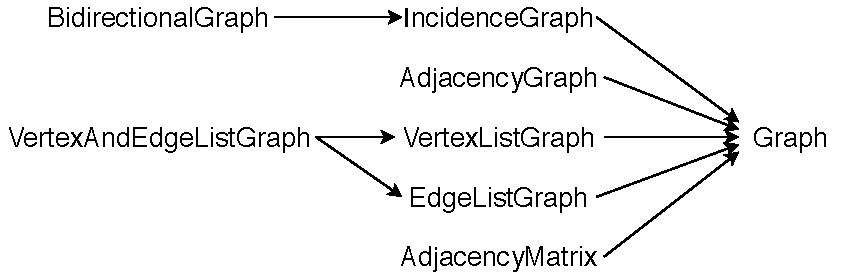
\includegraphics[width=1\textwidth]{img/graph-concepts.pdf}
 	\caption[The graph concepts and refinement relationships]{The graph concepts and refinement relationships (the image is taken from Boost website~\cite{graph_concepts}).}
 	\label{fig:graph_concepts}
\end{figure}

Bellow you can find a description for each graph concept from  \autoref{fig:graph_concepts}:\bigskip

\noindent\textbf{Graph concept}. This concept contains only a few requirements that are common for all other graph concepts. Examples of such requirements are \texttt{vertex\_descriptor} and \texttt{edge\_descriptor} (indices used to address vertices and edges, respectively).\bigskip

\noindent\textbf{AdjacencyGraph}. This concept provides efficient access to vertices adjacent to a certain vertex in the graph.\bigskip

\noindent\textbf{IncidenceGraph}. This concept provides efficient access to the out-edges of a certain vertex in the graph.\bigskip

\noindent\textbf{BidirectionalGraph}. This concept is similar to \emph{IncidenceGraph}, however it adds requirement for efficient access to in-edges. It is separated from \emph{IncidenceGraph}, because storing not only out-edges but also in-edges requires more storage space and not every algorithm requires in-edges (this is not an issue for undirected graphs, since every in-edge is also an out-edge).\bigskip

\noindent\textbf{AdjacencyMatrix}. This concept provides efficient access to any edge in the graph given the source and target vertices (this is achieved by storing edges in a matrix, hence the name \uv{Adjacency matrix}).\bigskip

\noindent\textbf{EdgeListGraph}. This concept provides efficient traversal of all edges in the graph, i.e., efficient iterating over every edge.\bigskip

\noindent\textbf{VertexListGraph}. This concept provides efficient traversal of all vertices in the graph, i.e., iterating over every vertex.\bigskip

\noindent\textbf{VertexAndEdgeListGraph}. This concept combines requirements of \emph{EdgeListGraph} and \emph{VertexListGraph}.

\subsection{Subgraph}\label{ssec:subgraph}
Lot of graph algorithms require the usage of subgraphs, in fact, even the implementation of a tree decomposition algorithm that we will discuss in the next chapter uses subgraphs. That is why BGL provides a class \texttt{subgraph} that is used to create subgraphs from a graph.

The \texttt{subgraph} class implements induced subgraphs. The main graph and its subgraphs are maintained in a tree data structure. The main graph is the root, and subgraphs are either children of the root or of other subgraphs. All of the nodes in this tree, including the root graph, are instances of the \texttt{subgraph} class. The \texttt{subgraph} implementation ensures that each node in the tree is an induced subgraph of its parent. The \texttt{subgraph} class implements the BGL \texttt{graph} interface, so each subgraph object can be treated as a graph~\cite{boost_subgraph}.

Example of a structure that maintains the parent graph and its subgraphs is shown in \autoref{fig:subgraph}. Each subgraph also has its own vertex and edge descriptor for each vertex and edge, respectively (called \emph{local}) as well as a \emph{global} descriptor, that is used to address the corresponding vertex or edge in the parent graph. That way we can distinguish between vertices and edges of the parent graph and its subgraphs.

\begin{figure}[H]
	\centering
	\subfloat[Graph $G$ and subgraphs $G1$, $G2$, and $G3$]{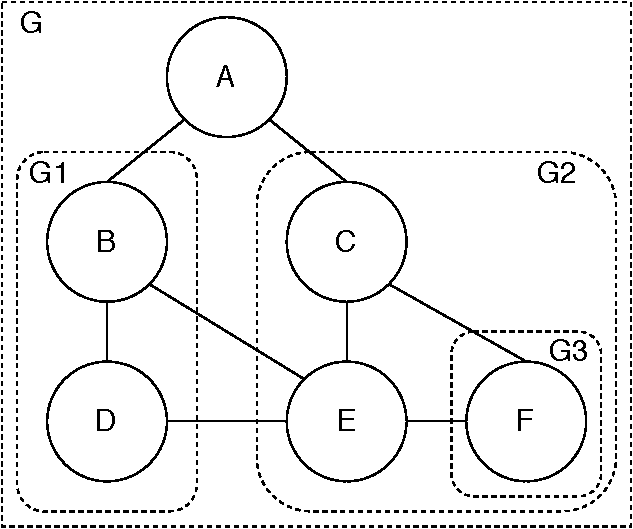
\includegraphics[width=8cm]{img/subgraph1.pdf}}
	\hspace{2em}
	\subfloat[Tree-like data structure of graph $G$ and its subgraphs]{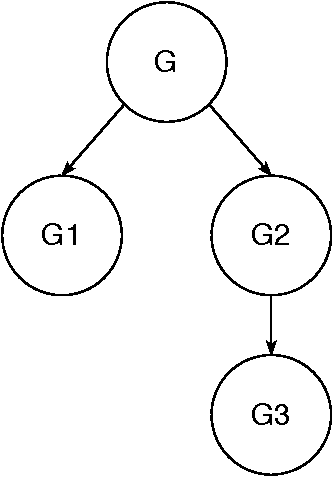
\includegraphics[width=4cm]{img/subgraph2.pdf}}
	\caption[Example of data representation used by class \texttt{subgraph}]{Example of data representation used by class \texttt{subgraph} to store graph $G$ with its subgraphs $G1$ and $G2$ (which has its own subgraph $G3$). Inspired by \cite{boost_subgraph_image}.}
	\label{fig:subgraph}
\end{figure}

\section{Notions of used algorithms}
In this section we will take a look at formal definitions of general and nice tree decomposition and get more familiar with their properties.
\subsection{Tree decomposition and treewidth}
\emph{Tree decomposition} is used to represent graph $G$ in a tree structure, allowing us to deduce certain connectivity properties. Also, as we already mentioned earlier, this decomposition is used to improve and speed up certain computationally complex algorithms---example of such an algorithm was given in the introduction of this thesis. We will discuss another example later on.\bigskip

\noindent Now onto the formal definition:

A \emph{tree decomposition} of a graph $G$ is pair $\mathcal{T} = (T, \{X_t\}_{t \in V(T)})$, where $T$ is a tree whose every node $t$ is assigned a vertex subset $X_t \subseteq V(G)$, called a \emph{bag}, such that the following three conditions hold:
\begin{enumerate}
    \item $\bigcup_{t \in V(T)} X_t = V(G)$. I.e., every vertex of $G$ is in at least one bag.
    \item For every $uv \in E(G)$, there exists a node $t$ of $T$ such that bag $X_t$ contains both $u$ and $v$.
    \item For every $u \in V(G)$, the set $T_u = \{t \in V(T) : u \in X_t \}$, i.e., the set of nodes whose corresponding bags contain $u$, induces a connected subtree of $T$.
\end{enumerate}

The \emph{width} of a \emph{tree decomposition} $\mathcal{T}$ is equals the size of its largest bag minus~1. The \emph{treewidth} of graph $G$ (denoted by tw($G$)) is the minimum possible width of a tree decomposition of graph $G$~\cite[Chap. 7.2]{param_algo}. See \autoref{fig:tree_decomposition} for an example. We will be using treewidth as a~parameter for an FPT algorithm\footnote{Fixed-parameter tractable (FPT) algorithm is an algorithm with complexity exponential only in the size of some fixed parameter $k$, therefore it works efficiently for a small~$k$.} provided by our library extension.

\begin{figure}[H]
	\centering
 	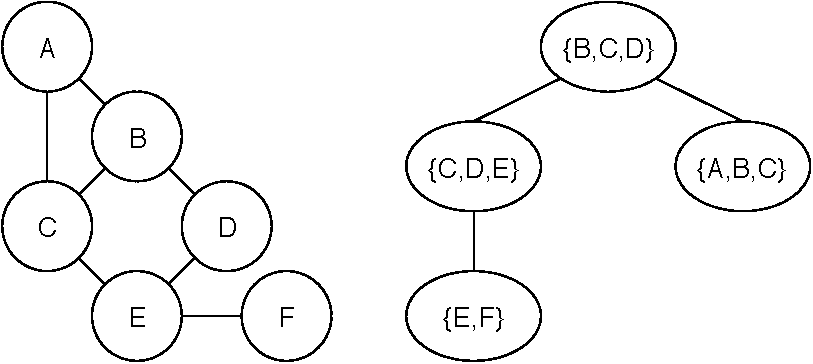
\includegraphics[width=8.8cm]{img/graph-decomposition.pdf}
 	\caption[Example of a graph and its tree decomposition]{Example of a graph (on the left) and its tree decomposition  of width 2 (on the right).}
 	\label{fig:tree_decomposition}
\end{figure}

\subsection{Nice tree decomposition} \label{ssec:nice_tree_decomposition}
Nice tree decomposition is a special type of a tree decomposition, that follows few more conditions in addition to those defined in previous subsection. Those conditions might seem unnatural, but they make the design of dynamic-programming algorithms much easier (as we will see in \autoref{sec:wis}), which is the primary motivation for introducing nice tree decompositions.

Important property of nice tree decompositions is that if a graph $G$ admits a tree decomposition of width $k$, then it also admits a nice tree decomposition of width $k$. In other words, every tree decomposition can be transformed into a nice tree decomposition without increasing its width~\cite[Lemma 7.4]{param_algo}.

We will say that a tree decomposition $\mathcal{T}$ rooted at $X_r$ is \emph{nice}, if following conditions are satisfied~\cite[Chapter 7.2]{param_algo}:
\begin{itemize}
	\item $X_r = \emptyset$ and $X_l = \emptyset$ for every leaf $l$ of $T$. In other words, all the leaves as well as the root contain empty bags.
	\item Every non-leaf node of $T$ is of one of the following three types:
	\begin{itemize}
		\item \textbf{Introduce node:} a node $t$ with exactly one child $t'$ such that \\ $X_t = X_{t'} \cup \{v\}$ for some vertex $v \notin X_{t'}$; we say that $v$ is \emph{introduced} at $t$.
		\item \textbf{Forget node:} a node $t$ with exactly one child $t'$ such that \\ $X_t = X_{t'} \setminus \{w\}$ for some vertex $w \in X_{t'}$; we say that $w$ is \emph{forgotten} at $t$.
		\item \textbf{Join node:} a node $t$ with two children $t_1$, $t_2$ such that \\ $X_t = X_{t_1} = X_{t_2}$.
	\end{itemize}
\end{itemize}

For an example of the nice tree decomposition of a tree decomposition presented in \autoref{fig:tree_decomposition} see \autoref{fig:nice_tree_decomposition}.

From now on, we will have to distinguish nice decomposition from \uv{not nice} decomposition. Decomposition that does not need to follow additional set of rules presented in this subsection will be referred to as an \emph{general tree decomposition}\footnote{Some publications use different term instead of a \uv{general tree decomposition}, e.g., \uv{simple tree decomposition}.}. The term \emph{tree decomposition} will be used as a generalization of both general and nice decompositions.

\begin{figure}[H]
	\centering
 	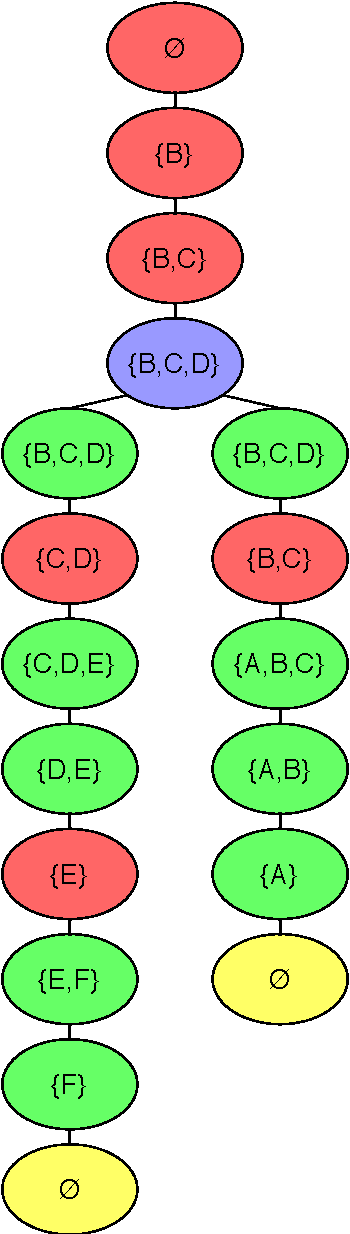
\includegraphics[width=3cm]{img/nice-graph-decomposition.pdf}
 	\caption[Example of a nice tree decomposition of the graph from  \autoref{fig:tree_decomposition}]{Example of a nice tree decomposition of the graph from  \autoref{fig:tree_decomposition} (root is on top, leaf nodes are yellow, introduce nodes green, forget nodes red, and the join node is blue).}
 	\label{fig:nice_tree_decomposition}
\end{figure}

\subsection{Maximum weighted independent set}
We will demonstrate the use of the library extension (specifically the nice tree decomposition) on the \textsc{Maximum Weighted Independent Set} problem, which can be described as follows (description is inspired by~\cite[Chap. 7.1]{param_algo}).

Imagine that you are a famous TV network hosting a large reality show with no capacity cap. You have already held a few auditions and rated each contestant with a score based on their \emph{fun factor}. Now it is up to you to select contestant, that will make the cut and will be participating in the reality show. When making the list of the cast, you would like to maximize the \emph{total fun factor} of the selected contestants. However you know that it is not a good idea to cast people that know each other, because they will most likely form a \uv{secret pact} giving them an unfair advantage against other contestants. That is why you will want to avoid this situation.

We model this problem as follows. Assume that relationships between contestants are represented by an undirected graph $G$. Vertices of $G$ represent contestants and each $v \in V(G)$ is assigned a non-negative weight $w(v)$ that represents the score (i.e., the \emph{fun factor}) given at the audition. Every edge $uv$ of $G$ represents that contestant $u$ knows contestant $v$ (this relation is symmetrical). The task is to find the maximum weight of an independent set in $G$. This problem is called \textsc{Maximum Weighted Independent Set}. For an example see \autoref{fig:mwis}.

\begin{figure}[H]
	\centering
 	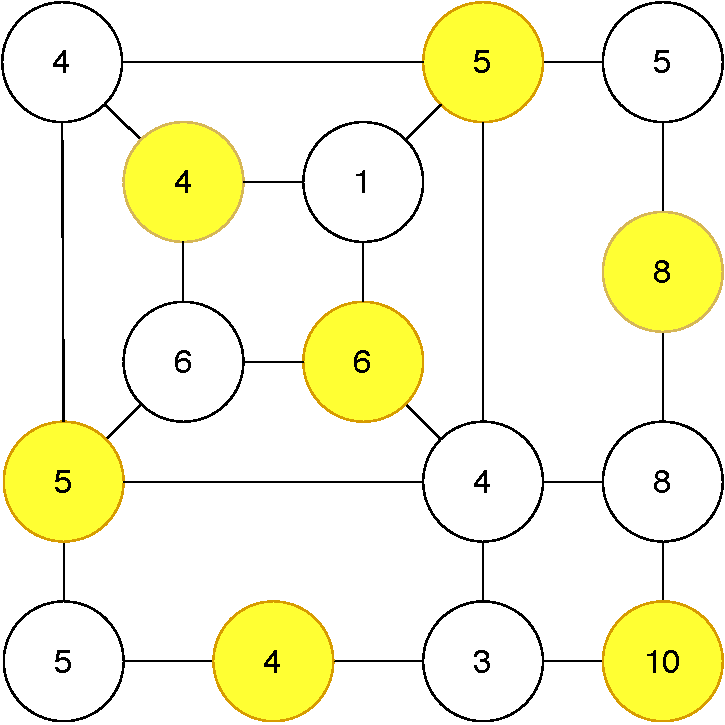
\includegraphics[width=8cm]{img/mwis.pdf}
 	\caption[Example of a graph and its maximum weighted independent set]{Example of a graph and its maximum weighted independent set (represented by yellow vertices) with total weight of 42.}
 	\label{fig:mwis}
\end{figure}

\chapter{Design}\label{chap:design}
Since we established the key algorithm notions and characteristics of BGL in previous chapter, we are ready to discuss requirements and code architecture of our library extension. This will also include introduction to the algorithms themselves---their core and used data structures.

\section{Requirement specification}\label{sec:requirment_specification}
In the analysis we discussed the importance of genericity and its impact on code design of whole BGL. On one hand, since this work is a BGL extension, it should follow the same principles---in other words, it should also be generic. Take the graph type as an example---we should not limit user to a certain type instance of \texttt{adjacency\_list}\footnote{\texttt{adjacency\_list} is specific class implementation of \emph{adjacency list} graph structure.}---instead, it should allow user to choose his own desired graph structure. On the other hand, we have to make sure our algorithm is compatible with any graph structure, which is often not possible. That is where concept checking\footnote{\url{https://www.boost.org/doc/libs/1_72_0/libs/concept_check/concept_check.htm}} comes in handy. BGL provides concept check library (BCCL), which adds a certain way for the writer of the function template to explicitly specify, \emph{which} model should the template argument (provided by user) conform to. This is achieved by \emph{concept asserts}, which cause compiler error message when incorrect template argument is supplied.

Same principle applies to the \emph{nice decomposition algorithm}. Instead of obtaining decomposition of certain graph inside, we will require a decomposition of a graph as an input and then transform the given decomposition into \emph{nice} one. That way the user can choose, which algorithm for retrieving tree decomposition he will use---be it the one provided in our BGL extension, or a different one.

There are a few more requirements, that will our library extension try to fulfil---those will be divided into functional and non-functional.

\subsection{Functional requirements}
\begin{enumerate}[F1)]
	\item Algorithm for obtaining a tree decomposition.
	\item Algorithm for turning a general tree decomposition into a nice one.
	\item Algorithm that uses dynamic programming over a tree decomposition.
	\item Each of algorithms should have generic interface that allows different types of graph as an input.
	\item If user provides incorrect input, algorithms should throw an exception or a compiler error.
	\item \emph{Nice decomposition algorithm} should allow user to select which tree decomposition algorithm will be applied.
\end{enumerate}

\subsection{Non-functional requirements}
\begin{enumerate}[N1)]
	\item Our library extension should follow Boost conventions (code-style, architecture, naming conventions, etc.)
	\item Only C++ Standard Library or other Boost libraries should be used.
	\item Documentation of algorithm interfaces should be provided.
	\item Majority of code should be covered by tests.
\end{enumerate}

\section{Architecture}
As mentioned in non-functional requirement specification (N1), code architecture should follow conventions of BGL. Since BGL is header-only library, the structure of our extension is quite simple and it consist only of header files. Each algorithm has its own separate file, that consist of various non-member functions which are part of \texttt{boost} namespace. Interface of each algorithm is directly accessible through that namespace. Other functions, that are not part of the interface and serve as \uv{helper} function inside the algorithm are inside another nested namespace \texttt{detail}, that is supposed to \uv{hide} the implementation from the user\footnote{This is an \uv{unspoken} convention used not only by BGL, please see discussion: \url{https://stackoverflow.com/questions/26546265/what-is-the-detail-namespace-commonly-used-for}}.

Each algorithm is covered by tests (Boost test library is used). Tests are located in separate directory, where each header file has its own test-file counterpart named \texttt{*headerfile\_name*\textbf{\_test.cpp}}. Every tested function has its own \emph{test suite}\footnote{\url{https://www.boost.org/doc/libs/1_72_0/libs/test/doc/html/boost_test/tests_organization/test_tree/test_suite.html}} which contains several test cases.

\section{Algorithm for obtaining a tree decomposition}\label{sec:algorithm_td}
Computing the treewidth of a given undirected graph is NP-hard~\cite{tree_decomposition_complexity} and there are many different approaches, e.g, exact or approximate fixed-parameter tractable (FPT) algorithms.

In this thesis we will be using the approximate FPT algorithm that mostly follows Reed~\cite{tree_decomposition_algorithm} and is described in the book \emph{Parameterized Algorithms}~\cite[Chap. 7.6.2]{param_algo}. Given an undirected graph $G$ and integer $k$, the task of this algorithm will be finding a tree decomposition of a graph $G$ with treewidth at most $3k+4$ or concluding that $tw(G) > k$. Time complexity of this algorithm is $\mathcal{O}(8^k k^2 n^2)$.

As a first step we will have to decide, whether given graph $G$ is connected or not. If it is not, we will apply the algorithm to each connected component of $G$ and connect obtained tree decompositions (see \autoref{fig:components_decomposition}). From now on, we will assume that $G$ is connected.

\begin{figure}[H]
	\centering
	\subfloat[Tree decompositions of components of graph $G$]{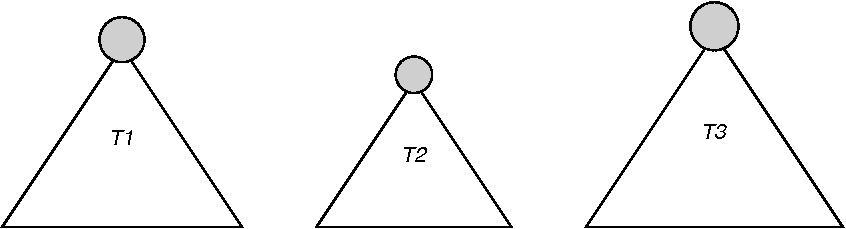
\includegraphics[width=6cm]{img/components-decomposition1.pdf}}
	\hspace{1em}
	\subfloat[Tree decomposition of a graph $G$]{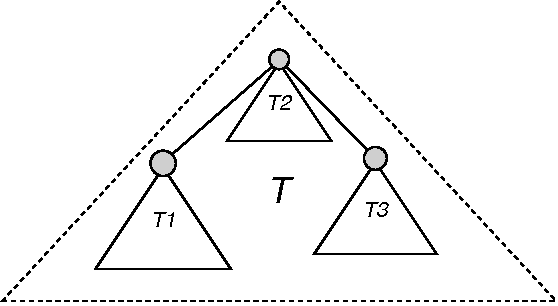
\includegraphics[width=6cm]{img/components-decomposition2.pdf}}
	\caption[Tree decomposition of a graph $G$ created by connecting decompositions of the components of $G$]{Tree decomposition of graph $G$ created by connecting decompositions of the components of $G$ (gray vertices are the root of they decomposition they belong to).}
	\label{fig:components_decomposition}
\end{figure}

The core of the algorithm will be a recursive procedure $decompose(W,S)$, where $S \subsetneq W \subseteq V(G)$ and $|S| \leq 3k+4$. This procedure tries to decompose subgraph $G[W]$ so that $S$ is contained in one of the bags of the decomposition. Output of this procedure will be a rooted tree decomposition $\mathcal{T}_{W,S}$. Root call of this procedure will be $decompose(V(G), \emptyset)$, which will return a rooted tree decomposition of~$G$.
\newpage
\subsection{Procedure decompose} \label{ssec:procedure_decompose}
First, we will need to construct a set $\widehat{S}$ with following properties:
\begin{enumerate}
	\item $S \subsetneq \widehat{S} \subseteq W$
	\item $|\widehat{S}| \leq 4k + 5$
	\item every connected component of $G[W \setminus \widehat{S}]$ is adjacent to at most $3k+4$ vertices of $\widehat{S}$.
\end{enumerate}
Constructed set $\widehat{S}$ will be the root bag of the decomposition constructed by this call of \emph{decompose}.

If $|S| < 3k+4$, we take any vertex $u \in W \setminus S$ and construct $\widehat{S}: S \cup \{u\}$. If $|S| = 3k+4$, we iterate through all possible partitions of $S$ into two parts $A$ and $B$ (there is $2^{3k+4}$ of them) and apply a max-flow algorithm to verify, whether minimum order of a separation of $G[W]$, where $A$ and $B$ are separated, does not exceed $k+1$. This is done by creating a new vertex, that will be connected with every vertex  of $A$---this will be the source for the max-flow algorithm. Similarly we will construct a new vertex connected with every vertex of $B$---this vertex will be the sink. After applying a max-flow algorithm to find a maximum flow between the newly created source and the sink, we will get a separation $(A',B')$, where $(A' \cap B')$ represents the cut.

If the computed flow is too big, i.e., such a partition of $S$ does not exist for every pair $(A,B)$, we can conclude that $tw(G[W]) > k$, therefore $tw(G) > k$ and we can terminate the whole algorithm. If we have found a partition $(A', B')$ that satisfies given properties, we can construct $\widehat{S}$ as $S \cup (A' \cap B')$.

After successfully constructing $\widehat{S}$, we create vertex sets $D_1,D_2,..,D_p$ for every connected component $i=1,2,..,p$ of $G[W \setminus \widehat{S}]$. For each $i$ we will recursively call $decompose(N_G[D_i], N_G(D_i))$ and let $r_i$ be the root of the decomposition returned by the decompose call. Now we will create root bag $X_r = \widehat{S}$ and for every $i$ we will attach each decomposition $\mathcal{T}_i$ below $r$ using edge $rr_i$ (note that if $p = 0$, then $\widehat{S}$ will be a leaf of the tree decomposition of $G$). We have successfully created decomposition of $\mathcal{T}_{w,s}$.

\subsection{Used data structures}\label{ssec:td_data_structures}
Now that we are familiar with the algorithm, our next aim will be choosing the right data representation. Since this work is a BGL extension, we will use existing solutions provided by the BGL.

In \autoref{ssec:graph_concepts} we discussed the role of graph concepts in BGL, which will now come handy. First step will be to decide, which type of a graph we expect as an input by user. In this algorithm we will need to traverse through all vertices many times (e.g., when we will need to retrieve all neighbours of a certain vertex or while constructing components of a given graph), therefore the best option is \emph{VertexListGraph}---it is the minimum concept, that includes the operation we will require.

Second step will be to decide which type of a graph will be used to represent the tree decomposition. As opposed to the input graph, we do not require any special operations on this graph---only required operations are adding vertices and edges, which are basic operations supported by every graph concept. Therefore there is no point in limiting user to certain graph concept and we will let him decide, which one he wants to use.

Last step will be choosing the right data structure to represent bags of the decomposition. Since it is more complex, we will dedicate a separate section for it (see \autoref{sec:bags_representation}).

\section{Algorithm for obtaining a nice tree decomposition}\label{sec:ntd_algorithm}
Main task of this algorithm will be creating a nice tree decomposition $d_2$ from an general tree decomposition $d_1$ provided by the user. This will be done by traversing through graph $d_1$ while simultaneously constructing graph $d_2$ that follows additional set of rules introduced in the definition of the nice tree decomposition (see \autoref{ssec:nice_tree_decomposition}).

Algorithm is described in \autoref{fig:ntd_activity_diagram}. Note that UML activity diagram is significantly simplified in order to maintain readability. From the diagram we can observe that constructing a nice decomposition from a general decomposition will not affect its width, i.e., if a decomposition $d_1$ has width $k$, decomposition $d_2$ will also have width~$k$~\cite[Chap. 7.2]{param_algo}. To really simplify the algorithm, first, we will construct node with empty bag for every leaf node of $d_1$. Second, we will insert a few nodes between each other nodes of $d_1$ where each time there will be one element from node of $d_1$ introduced or forgotten. That way we will never construct a node with a bag that has more elements than the largest bag of $d_1$, causing the increased width of $d_2$.

\begin{figure}
	\centering
 	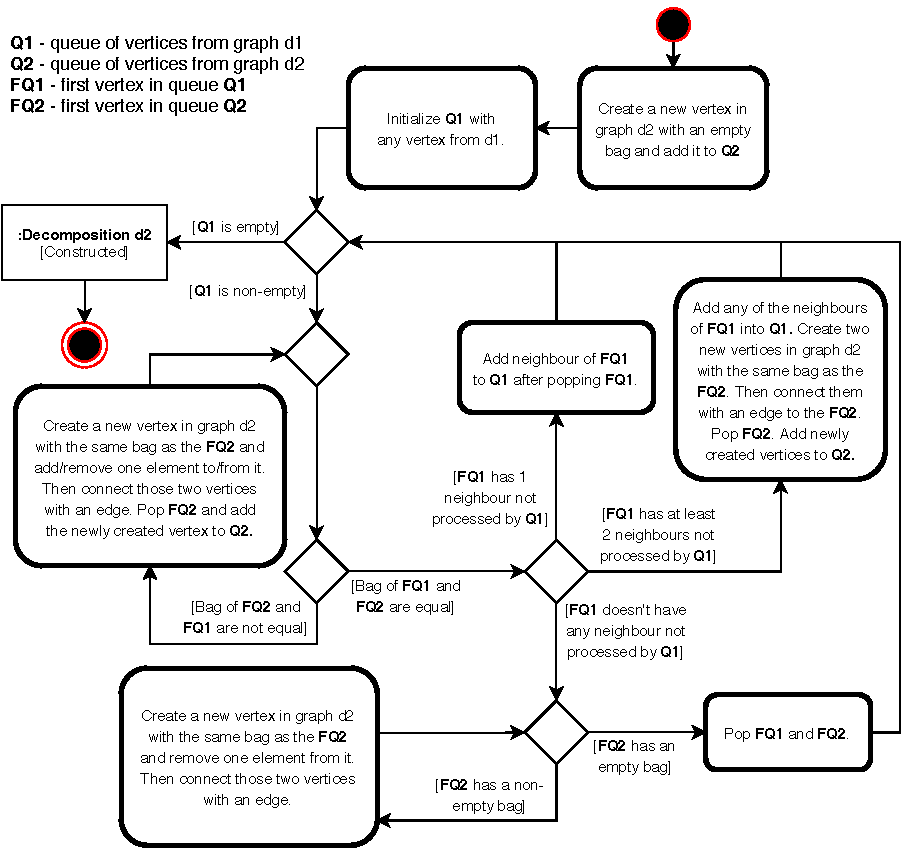
\includegraphics[width=1\textwidth]{img/ntd-activity-diagram.pdf}
 	\caption[UML activity diagram describing construction of the nice decomposition]{UML activity diagram describing construction of the nice decomposition (graph $d1$ is a general decomposition provided by user and graph $d2$ is a nice tree decomposition).}
 	\label{fig:ntd_activity_diagram}
\end{figure}

\subsection{Used data structures}\label{ssec:ntd_data_structures}
Data representation will be similar to the one used in the algorithm for obtaining a general tree decomposition. However this time we will not require a~graph whose nice decomposition we will be constructing, just the general decomposition.

We will have to decide, which type of graph we will use for both types of decomposition. Since we will be traversing through the vertices of a general decomposition provided by the user, \emph{VertexListGraph} will be the best option.

Similarly to the general decomposition algorithm, the data structure to represent the bags of both decompositions will be discussed in \autoref{sec:bags_representation}.

\section{Representation of mutable bags}\label{sec:bags_representation}
Since we want to give the user as much freedom of choice as possible, we will use something called \emph{Read/Write Property Map}\footnote{\url{https://www.boost.org/doc/libs/1_72_0/libs/property_map/doc/ReadWritePropertyMap.html}}---it is a generic interface for associative map, that allows read and write operations (value is retrieved using the key). That way the user can choose a data structure (e.g., \texttt{std::map}) as long as it follows the rules of \emph{Read/Write Property Map} concept. The value type of this map will be a mutable container. Graphical illustration of this data structure is presented in \autoref{fig:bags_representation}.

\begin{figure}[H]
	\centering
 	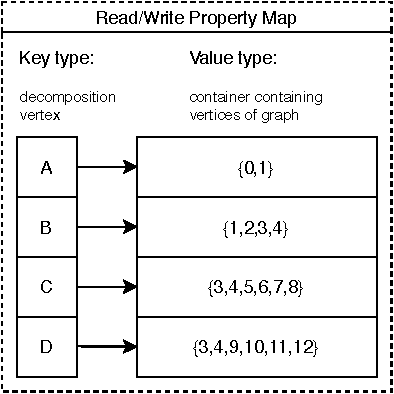
\includegraphics[width=10cm]{img/bags-representation.pdf}
 	\caption[Graphical illustration of data structure that represents bags]{Graphical illustration of data structure that represents bags.}
 	\label{fig:bags_representation}
\end{figure}

Next step will be choosing the right concept of a container that will represent a single bag of node of the decomposition (we will be using list of concepts provided by BGL as a reference~\cite{boost_concepts}). BGL offers a wide range of concepts and the most basic and simple one is \emph{Collection}\footnote{\url{https://www.boost.org/doc/libs/1_72_0/libs/utility/Collection.html}}. It provides methods for accessing and most importantly iterating over the container. However it does not provide a method for inserting elements into the container, which is one of the key methods that we will need (since we will be constructing bags, which requires inserting of elements). Therefore \emph{Collection} concept is not suitable for us.

The most basic concept that provides \emph{insert} method is \emph{Sequence}\footnote{\url{https://www.boost.org/sgi/stl/Sequence.html}}. However downside of this concept is that it does not support popular containers like \texttt{std::set} or \texttt{std::unordered\_set}.

Since none of the concepts provided by BGL is entirely suitable, we will have to define our own container concept called \emph{InsertCollection}. Its implementation will be discussed in \autoref{sec:insertcollection}.

\section{Maximum weighted independent set algorithm}\label{sec:wis}
Solving the \textsc{Maximum Weighted Independent Set} problem is classified as NP-hard~\cite{mwis_np}. For the naive brute-force approach we would have to generate every possible set of vertices of graph $G$ (that is $2^n$ permutations) and find the maximum weighted independent set among them---that would result into time complexity $\mathcal{O}(2^n \cdot n^2)$.

However we can approach this problem much more effectively provided that we have a nice tree decomposition $\mathcal{T} = (T, \{X_t\}_{t \in V(t)})$ of graph $G$ of width $k$ with root $r$. We will be using the algorithm described in the book \emph{Parameterized Algorithms}~\cite[Chap. 7.3.1]{param_algo}. This algorithm will allow us to solve problem in time $2^k \cdot k^{\mathcal{O}(1)}$. The core of the algorithm will be a bottom-up dynamic programming based procedure \emph{calculate\_weight(t, S)}:

\begin{center}
\centering
\emph{calculate\_weight(t, S)} = maximum possible weight of the set $\widehat{S}$ such that

$S \subseteq \widehat{S} \subseteq V_t$, $\widehat{S} \cap X_t = S$, and $\widehat{S}$ is independent, where $V_t$ is the union of all the bags present in the subtree of $T$ rooted at $t$, including $X_t$
\end{center}

If no such set $\widehat{S}$ exists (for example $S$ itself is not independent), the return value of the procedure will be $-\infty$. Root call of the procedure will be \emph{calculate\_weight(r, $\emptyset$)}, which will calculate the maximum weight of graph $G$, because $V_r = V(G)$.

\subsection{Procedure calculate\_weight}\label{ssec:mwis_calculate_weight}
This recursive procedure defines behaviour for each type of node $t$ we will be possibly dealing with. The base case of this recurrence will be the leaf node. For  non-leaf nodes, the result of the procedure depends on the results of their child nodes. Now we will define the behaviour for each type of nodes introduced in \autoref{ssec:nice_tree_decomposition} (in order to retain readability, we will be using the abbreviation \emph{cw} instead of full name of the procedure):\bigskip

\noindent\textbf{Leaf node}. If $t$ is a leaf node, we will return $0$.\medskip

\noindent\textbf{Introduce node}. If $t$ is an introduce node with a child $t'$ such that \linebreak $X_t = X_{t'} \cup \{v\}$ for some $v \not\in X_{t'}$, we put:

\begin{equation}
cw(t, S) = 
	\begin{cases}
		cw(t', S) & \text{if $v \not\in S$}\\
		cw(t', S \setminus \{v\}) + w(v) & \text{if $S \setminus \{v\}$ is independent}\\
		-\infty & \text{otherwise}
	\end{cases}
\end{equation}

\noindent\textbf{Forget node}. If $t$ is a forget node with a child $t'$ such that $X_t = X_{t'} \setminus \{w\}$ for some $w \in X_{t'}$, we put:

\begin{equation}
cw(t, S) = \text{max} \left\{ cw(t',S), cw(t', S \cup \{ w \}) \right\}
\end{equation}

\noindent\textbf{Join node}. If $t$ is a join node with children $t_1,t_2$ such that $X_t = X_{t_1} = X_{t_2}$, we put:

\begin{equation}
cw(t,S) = cw(t_1,S) + cw(t_2,S) - w(S)
\end{equation}

\subsection{Used data structures}\label{ssec:mwis_data_structure}
Now we can move onto the choosing of right data structures. Most of them will be similar to those used in previous algorithms.

First we need to choose the right representation for both graph and its nice decomposition. In both cases we will need to traverse through vertices---as we already established in previous sections, best graph concept for this matter is \emph{VertexListGraph}. Both of these graphs can be of different type, however they both have to implement the graph concept \emph{VertexListGraph}.

Next are the bags of the decomposition. Since the algorithm will use the bags of decomposition only for reading, they will be be represented by \emph{Readable Property Map}. The value type of the map will be \emph{Container}\footnote{\url{https://www.boost.org/sgi/stl/Container.html}}, which is the most generic interface for a container that provides basic operations for~reading. 

Each of the vertices of the graph should have defined its weight. For this we will be using similar approach as we did with bags, that is, \emph{Read/Write Property Map}, where we will use the vertex descriptor as a key to access the weight of the said vertex. However the weight has to be a non-negative integer (e.g., \texttt{uint}, \texttt{ulong}).

The purpose of this algorithm is not only to return the total weight of the found maximal weighted set, but also provide the set itself. This will be achieved by using something called \emph{Color Map}---it is basically another \emph{Property Map}, where each vertex of a graph has assigned a color\footnote{\url{https://www.boost.org/doc/libs/1_72_0/libs/graph/doc/ColorValue.html}}. In our case we will use two colors---white, if vertex belongs to the maximal weighted set or black otherwise.

\chapter{Implementation}\label{chap:implementation}
This chapter will focus on fulfilling functional and non-functional requirements from the previous chapter. It will be divided into three sections (for each algorithm mentioned in F1, F2, and F3). In each of these parts we will discuss interface, core of the functions and reasoning behind certain decisions that were made.

\section{Algorithm for obtaining a tree decomposition}\label{sec:td_implementation}
In this section we will focus on implementation of the algorithm that constructs general tree decomposition---function \texttt{tree\_decomposition}. Interface of the function is shown in \autoref{lst:tree_decomposition_interface}.

\begin{listing}[H]
	\inputminted[tabsize=2,breaklines,bgcolor=codebg]{c++}{snippets/tree_decomposition_interface.m}
	\caption[Interface of the function \texttt{tree\_decomposition}]{Interface of the function \texttt{tree\_decomposition}.}
	\label{lst:tree_decomposition_interface}
\end{listing}

\noindent\texttt{Graph \textbf{g}}---graph whose tree decomposition will be constructed.

\noindent\texttt{Decomposition \textbf{d}}---graph in which will be the decomposition stored (this is an in/out parameter).

\noindent\texttt{Bags \textbf{bags}}---\emph{Property Map} containing bags for each node of \texttt{d} (this is an in/out parameter).

\noindent\texttt{unsigned long \textbf{k}}---parameter, which will limit the width of decomposition.

Return value of this function will be a boolean---\emph{true}, if tree decomposition of graph \texttt{g} exists with width at most $3k+4$ and \emph{false} if such a decomposition does not exist.

Since most of the parameters of the function are template parameters, we have to assure that the user provided a correct input (preferably during compilation). That is achieved using the \emph{Boost concept asserts} and \emph{Boost static asserts}. If any of these asserts (see \autoref{lst:tree_decomposition_asserts}) fails, then compilation error will be thrown.

\begin{listing}[H]
	\inputminted[tabsize=2,breaklines,bgcolor=codebg]{c++}{snippets/tree_decomposition_asserts.m}
	\caption[Asserts of the function \texttt{tree\_decomposition}]{Asserts of the function \texttt{tree\_decomposition}.}
	\label{lst:tree_decomposition_asserts}
\end{listing}

\begin{itemize}
	\item [A1)] \emph{Graph} must be a model of \emph{VertexListGraphConcept}.
	\item [A2)] Each bag of \emph{Bags} container must be a model of \emph{InsertCollection} (see \autoref{sec:insertcollection}).
	\item [A3)] \emph{Bags} must be a model of \emph{Read/Write Property Map} (with \emph{Decomposition} vertex descriptor as a key).
	\item [A4)] \emph{Graph} vertex descriptor and value type of container inside the \emph{Bags} must be the same type.
\end{itemize}

\subsection{Implementation of the algorithm}
Now that we are familiar with the interface of the function, let us take a closer look into the implementation. 

Assuming that all concept asserts passed, next step will be retrieving all connected components of graph \emph{g} provided by user, since procedure \emph{decompose} expects sets of vertices from a connected graph. This is achieved by helper function \texttt{get\_components}, which returns all components of \emph{g} in a \texttt{std::vector}. However this function requires \texttt{subgraph} (see chapter \autoref{ssec:subgraph}) as an input, so we have to create empty instance of class \texttt{subgraph} and copy graph \emph{g} into it.

Then, function \texttt{decompose} is called on every component. Return type of this function is \texttt{boost::tuple}, where first element is \texttt{vertex\_descriptor} of root node of decomposition, that was constructed by current call of \texttt{decompose} and the second one is bool. If the bool = \emph{true}, decomposition was found. Otherwise, decomposition was not found and we can immediately return \emph{false} without further inspection of remaining components.

If the decomposition of every component was successfully found, we will connect each decomposition with an edge to create one connected decomposition. Now we can return \emph{true}, since decomposition of \emph{g} was found and successfully~constructed.

\subsection{Procedure decompose}
Function \texttt{decompose} is the core and also the most important part of this algorithm. By recursively calling this function, decomposition of graph \emph{g} and its bags will be constructed (both \emph{decomposition} and \emph{Property Map} representing the bags are passed by reference). First (aka the root) call of this recursive function will contain empty decomposition, empty bags, \texttt{std::set} of vertex descriptors \emph{w} containing all vertices of graph \emph{g} and empty \texttt{std::set} \emph{s}.

First goal of this function is to construct set \emph{s1} (corresponding to the set $\widehat{S}$ in \autoref{ssec:procedure_decompose}). If size of set \emph{s} is smaller than $3k + 4$, we iterate over set \emph{w} in order to find a vertex that is not contained in \emph{s} and to insert it into set \emph{s}---this is done by trying to emplace every vertex of \emph{w} into \emph{s} using \texttt{std::set.emplace()}. If enough vertices were successfully inserted, we stop iterating and carry on with the algorithm.

If the size of \emph{s} is equal to $3k + 4$, we have to find a vertex separation of \emph{s} in graph \emph{g} with minimum order not exceeding $k+1$. Such a separation is retrieved using the helper function \texttt{get\_separation} that returns either a set of vertices forming the desired separation or an empty set if such separation was not found---in that case, we can immediately return \emph{false} in the current call of \texttt{decompose}, since decomposition of width $\leq 3k+4$ cannot be constructed.
\newpage
Now we can insert a new vertex into the decomposition graph---it will represent the root node of the decomposition created by the current call of \texttt{decompose}. Since every node of \emph{decomposition} should have its own bag, we will create a new bag for this node and it will contain all vertices from set \emph{s1}.

Finally, we will create a new subgraph of \emph{g}, that will contain vertices from $w \setminus s$ (we will call this set \emph{d} in short). This can be easily done by using \texttt{std::set\_difference}---it inserts difference of two sets into a new one, in our case set \emph{d}. Next, we will construct a new subgraph \emph{d\_graph} using the set of vertices \emph{d} obtained earlier. Now we can call recursively \texttt{decompose} on every component of \emph{d\_graph} (see \autoref{lst:decompose_rec}).

\begin{listing}[H]
	\inputminted[tabsize=2,breaklines,bgcolor=codebg]{c++}{snippets/decompose_rec.m}
	\caption[Creation of new recursive calls of the function \texttt{decompose}]{Creation of new recursive calls of the function \texttt{decompose}.}
	\label{lst:decompose_rec}
\end{listing}

\subsection{Retrieving separation}\label{ssec:retrieving_separation}
Function \texttt{get\_separation} is another very important helper function. Its main purpose is to find a vertex separator of a graph containing vertices from \emph{s} with minimum order not exceeding $k+1$. If such a separator does not exist, an empty set will be returned.

First, we will need to generate every possible partition of $s$ into two non-empty parts. This is done by the function \texttt{split\_set}, which takes a set of vertices $s$ and a seed number \emph{c\_number} and returns a tuple of two sets (let us call them $a$ and $b$). Binary representation of \emph{c\_number} will decide, how $s$ will be divided: If $n$th number of the binary representation of \emph{c\_number} is \texttt{0}, the $n$th element of $s$ will belong to $a$. Otherwise it will belong to $b$. Implementation of this function is shown in \autoref{lst:split_set}.

\begin{listing}[H]
	\inputminted[tabsize=2,breaklines,bgcolor=codebg]{c++}{snippets/split_set.m}
	\caption[Implementation of the function \texttt{split\_set}]{Implementation of the function \texttt{split\_set}.}
	\label{lst:split_set}
\end{listing}

Now that we have every possible partition of $s$, we can move onto finding a minimum separator that separates $a$ and $b$. This is achieved by function \texttt{max\_flow\_sep} that applies max-flow algorithm on a graph $g$, where partition $a$ will be the source and partition $b$ will be the sink, which calculates the vertex separation of the partition (this will be our desired separator). For that, we will be using \texttt{edmonds\_karp\_max\_flow} provided by BGL that implements Edmonds and Karp algorithm. However this leads to a few obstacles which will force us to slightly modify the graph $g$ before using \texttt{edmonds\_karp\_max\_flow}.

First obstacle is that \texttt{edmonds\_karp\_max\_flow} expects directed graph as an input---however we are working with undirected graphs (see \autoref{sec:algorithm_td}). This is easily solved by converting our graph $g$ into a new one (let us call it~\emph{g1}) where every undirected edge $uv$ will be represented by two directed edges $uv$ and $vu$. From now on we will be working with a newly created graph \emph{g1}.

Second obstacle is that \texttt{edmonds\_karp\_max\_flow} calculates an edge separator instead of a vertex separator. For each vertex $v$ we will create two vertices $v_1$ and $v_2$ connected by directed edge $v_1v_2$. Every edge that had an end in $v$ will be connected to $v_1$ and every edge that had a start in $v$ will be connected to $v_2$ (see \autoref{fig:vertex_edge_representation}). This method is explained in a proof of Menger theorem~\cite{menger_proof}. Now if the max-flow algorithm calculates an edge $v_1v_2$ as a part of separator of $g1$, it means that vertex $v$ is also a part of separator of a graph $g$. 

\begin{figure}[H]
	\centering
 	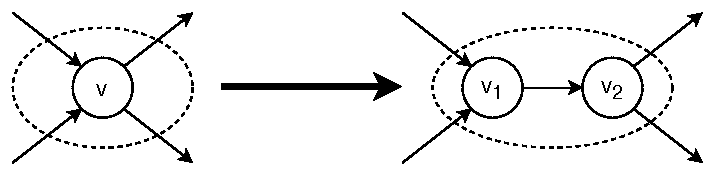
\includegraphics[width=10cm]{img/vertex-edge-representation.pdf}
 	\caption[\uv{Simulating} a vertex $v$ with an edge $v_1v_2$]{\uv{Simulating} a vertex $v$ with an edge $v_1v_2$.}
 	\label{fig:vertex_edge_representation}
\end{figure}

Our source for the max-flow algorithm is a set $a$ and the sink is a set $b$. Both of these sets can contain multiple vertices, however \texttt{edmonds\_karp\_max\_flow} expects a single vertex as a source and sink. As described in \autoref{ssec:procedure_decompose}, we will have to create two new vertices $x_1$ and $x_2$ in a graph $g1$, representing the source and sink, respectively. Vertex $x_1$ will be connected with every vertex of $a$ and $x_2$ will be connected with every vertex of $b$.

As a last step, we have to define capacities for each edge of $g1$. Edges that \uv{simulate} a vertex from $g$ (described in \autoref{fig:vertex_edge_representation}) will have capacity set to \texttt{1}. Every other edge has capacity of \texttt{2} (thus these edges will not be part of the computed separator). Capacities are stored in \emph{Property Map}, that is passed as an argument to~\texttt{edmonds\_karp\_max\_flow}.

Now we are ready to call \texttt{edmonds\_karp\_max\_flow}. If the return value of this function is at most $k+1$, we have successfully found separation of a graph $g1$---edges of this separation are stored in another \emph{Property Map}. For each edge $v_1v_2$ contained in \emph{Property Map} we will insert vertex $v$ from $g$ into the set, that will be the return value of function \texttt{get\_separation}. This set is our desired vertex separation of graph $g$.

If the return value of \texttt{edmonds\_karp\_max\_flow} is higher than $k+1$, function \texttt{max\_flow\_sep} will return an empty set and it will have to be called on another partition of $s$ created by the function \texttt{split\_set}.

\subsection{Retrieving components}
Earlier we mentioned helper function \texttt{get\_components} that is used to retrieve all components of a certain subgraph $G$. This function is basically a wrapper around \texttt{boost::connected\_components} provided by BGL, which returns number of all components and a map where each vertex from $G$ has assigned an integer which determines in which component it belongs to. However this representation is not suitable for our algorithms, therefore we will rewrite the map into \texttt{std::vector} containing pointers to all of the components of graph~$G$.

\subsection{Retrieving neighbours}
Another useful helper function is \texttt{get\_neighbour\_vertices} which returns all of the neighbour vertices of a subgraph $G'$ in a parent graph $G$ (formally $N_G[G']$ or $N_G(G')$).

It is basically a wrapper around the function \texttt{boost::adjacent\_vertices} provided by BGL with a small modification---our function takes in addition to subgraph $G'$ also a boolean as an input which determines if the neighbours of $G'$ should also include vertices of $G'$ themselves. If the boolean is set to \emph{true}, vertices of $G'$ are included, otherwise they are not (formally $N_G[G']$ and $N_G(G')$, respectively).

\section{Algorithm for obtaining a nice tree decomposition}\label{sec:ntd_implementation}
In \autoref{sec:ntd_algorithm} we discussed the algorithm that constructs a nice decomposition based on a general tree decomposition provided by the user and now it is time to take a look at the implementation. Interface of the function \texttt{nice\_tree\_decomposition} is shown in \autoref{lst:nice_tree_decomposition_interface}. Note that both general and nice tree decomposition use the same data type for the graph and its~bags.

\begin{listing}[H]
	\inputminted[tabsize=2,breaklines,bgcolor=codebg]{c++}{snippets/nice_tree_decomposition_interface.m}
	\caption[Interface of the function \texttt{nice\_tree\_decomposition}]{Interface of the function \texttt{nice\_tree\_decomposition}.}
	\label{lst:nice_tree_decomposition_interface}
\end{listing}

\noindent\texttt{Decomposition \textbf{d}}---a general decomposition based on which a nice tree decomposition will be constructed.

\noindent\texttt{Bags \textbf{bags}}---\emph{Property Map} containing bags for each node of \texttt{d}.

\noindent\texttt{Decomposition \textbf{nice\_d}}---graph in which will be the constructed nice decomposition stored (this is an in/out parameter).

\noindent\texttt{Bags \textbf{nice\_bags}}---\emph{Property Map} containing bags for each node of \texttt{nice\_d} (this is an in/out parameter).

Return value of this function is \texttt{vertex\_descriptor} of root node of constructed decomposition. If \texttt{d} contains a cycle, \texttt{std::invalid\_argument} exception is thrown.

Similarly to function \texttt{tree\_decomposition} we have to make sure that user provided a correct input. For example if graph concept that does not support traversing through vertices was provided, code would not compile and compiler would produce long error messages, making it much harder for user to find out what he did wrong---this is why we will use \emph{Boost concept asserts}. Below is a list of all used asserts (for more details see \autoref{lst:nice_tree_decomposition_asserts}):

\begin{itemize}
	\item [A1)] \emph{Decomposition} must be a model of \emph{VertexListGraphConcept}.
	\item [A2)] Each bag of \emph{Bags} container must be a model of \emph{InsertCollection} (see \autoref{sec:insertcollection}).
	\item [A3)] \emph{Bags} must be a model of \emph{Read/Write Property Map} (with \emph{Decomposition} vertex descriptor as a key).
\end{itemize}

\begin{listing}[H]
	\inputminted[tabsize=2,breaklines,bgcolor=codebg]{c++}{snippets/nice_tree_decomposition_asserts.m}
	\caption[Asserts of the function \texttt{nice\_tree\_decomposition}]{Asserts of the function \texttt{nice\_tree\_decomposition}.}
	\label{lst:nice_tree_decomposition_asserts}
\end{listing}

\subsection{Implementation of the algorithm}
In \autoref{sec:ntd_algorithm} we have gotten familiar with a simplified version of this algorithm (especially in \autoref{fig:ntd_activity_diagram}). Actual implementation is similar, however instead of an iterative algorithm with a queue we will be using a recursive function \texttt{nice\_decomposition\_rec}, that works in the same manner. In the next few paragraphs we will be using same terms, as in \autoref{sec:ntd_algorithm}---$d_1$ is a general decomposition, $d_2$ is a nice decomposition, \emph{FQ1} and \emph{FQ2} is (since we do not use a queue) a currently processed vertex from $d_1$ and $d_2$, respectively.

Function \texttt{nice\_decomposition\_rec} takes \emph{FQ1} and \emph{FQ2} as a parameter, compares them and if there are any differences between their bags, new vertex is constructed in $d_2$ and \texttt{nice\_decomposition\_rec} is called with a new \emph{FQ2}. If there are no differences, we can move on to another vertex from $d_1$ (this vertex will be a new \emph{FQ1}).

The root call of \texttt{nice\_decomposition\_rec} will be with a vertex that has an empty bag as \emph{FQ2} (this will be also the root of $d_2$) and any vertex from $d_1$ as \emph{FQ1} (it does not matter which one since $d_1$ is not rooted).

After \texttt{nice\_decomposition\_rec} successfully finishes, $d_2$ will contain a nice tree decomposition constructed based on $d_1$. Then the root of $d_2$ is returned as a return value of the function \texttt{nice\_tree\_decomposition}.

\section{Concept InsertCollection}\label{sec:insertcollection}
In \autoref{sec:bags_representation} we discussed the reason behind defining our own container concept and now it is time to take a look at the implementation (presented in \autoref{lst:insertcollection}). The implementation will be following \emph{Boost Concept Check Library} (BCCL) standards~\cite{bccl_class}.

\begin{listing}[H]
	\inputminted[tabsize=2,breaklines,bgcolor=codebg]{c++}{snippets/insertcollection.m}
	\caption[Definition of concept \emph{InsertCollection}]{Definition of concept \emph{InsertCollection}.}
	\label{lst:insertcollection}
\end{listing}

\emph{InsertCollection} is defined using \texttt{struct} that is a refinement of BCCL concept \emph{Collection}---this ensures that any data structure that is in conformance to \emph{InsertCollection} is also in conformance to \emph{Collection}. Inside \texttt{struct} we will use macro \texttt{BOOST\_CONCEPT\_USAGE} that exercises if method \emph{insert} is defined for the data structure that is being tested. If it is undefined, substitution of template argument \texttt{C} will fail and the code will not compile. Interface of method \texttt{insert} must be defined as follows:

\begin{center}
\centering
\texttt{insert ( iterator pos, T\& value );}
\end{center}

Iterator \texttt{pos} is a position where the element \texttt{value} should be inserted (in case of sorted container it is as close to \texttt{pos} as possible). Return value is not tested. This interface was chosen because it is implemented by most of the containers of \emph{C++ Standard Library}. For summary of containers that implement this interface refer to \autoref{tab:insert_containers}.

\begin{table}[h]
\centering
\begin{tabular}{|l|l|l|}
\hline
\textbf{Container} & \textbf{Implements \texttt{insert}?} & \textbf{Since} \\ \hline
\texttt{std::array} & \cellcolor[HTML]{FF8E8A}No & - \\
\texttt{std::vector} & \cellcolor[HTML]{9AFF99}Yes & C++11~\cite{std_vector} \\
\texttt{std::deque} & \cellcolor[HTML]{9AFF99}Yes & C++11~\cite{std_deque} \\
\texttt{std::forward\_list} & \cellcolor[HTML]{FF8E8A}No & - \\
\texttt{std::list} & \cellcolor[HTML]{9AFF99}Yes & C++11~\cite{std_list} \\
\texttt{std::set} & \cellcolor[HTML]{9AFF99}Yes & C++11~\cite{std_set} \\
\texttt{std::map} & \cellcolor[HTML]{9AFF99}Yes & C++11~\cite{std_map} \\
\texttt{std::multiset} & \cellcolor[HTML]{9AFF99}Yes & C++11~\cite{std_multiset} \\
\texttt{std::multimap} & \cellcolor[HTML]{9AFF99}Yes & C++11~\cite{std_multimap} \\
\texttt{std::unordered\_set} & \cellcolor[HTML]{9AFF99}Yes & C++11~\cite{std_unordered_set} \\
\texttt{std::unordered\_map} & \cellcolor[HTML]{9AFF99}Yes & C++11~\cite{std_unordered_map} \\
\texttt{std::unordered\_multiset} & \cellcolor[HTML]{9AFF99}Yes & C++11~\cite{std_unordered_multiset} \\
\texttt{std::unordered\_multimap} & \cellcolor[HTML]{9AFF99}Yes & C++11~\cite{std_unordered_multimap} \\
\texttt{std::stack} & \cellcolor[HTML]{FF8E8A}No & - \\
\texttt{std::queue} & \cellcolor[HTML]{FF8E8A}No & - \\
\texttt{std::priority\_queue} & \cellcolor[HTML]{FF8E8A}No & - \\ \hline
\end{tabular}
\caption[Summary of \emph{C++ Standard Library} containers and their support of the interface of method \texttt{insert} defined in \emph{InsertCollection} concept]{Summary of \emph{C++ Standard Library} containers and their support of the interface of method \texttt{insert} defined in \emph{InsertCollection} concept.}
\label{tab:insert_containers}
\end{table}

\section{Maximum weighted independent set algorithm}\label{sec:mwis}
In this section we will focus on implementation of the algorithm that solves the \textsc{Maximum Weighted Independent Set} problem---i.e., the function \texttt{max\_weighted\_independent\_set}. Interface of the function is shown in \autoref{lst:mwis_interface}.

\begin{listing}[H]
	\inputminted[tabsize=2,breaklines,bgcolor=codebg]{c++}{snippets/mwis_interface.m}
	\caption[Interface of the function \texttt{max\_weighted\_independent\_set}]{Interface of the function \texttt{max\_weighted\_independent\_set}.}
	\label{lst:mwis_interface}
\end{listing}
\newpage
\noindent\texttt{Graph \textbf{g}}---graph whose maximum weighted independent set will be computed.

\noindent\texttt{Decomposition \textbf{d}}---nice tree decomposition of graph \texttt{g}.

\noindent\texttt{Bags \textbf{bags}}---\emph{Property Map} containing bags for each node of \texttt{d}.

\noindent\texttt{decomposition\_vertex\_descriptor \textbf{root}}---root node of decomposition \texttt{d}.

\noindent\texttt{Weights \textbf{weights}}---\emph{Property Map} that contains weights for each vertex of \texttt{g}.

\noindent\texttt{Colors \textbf{colors}}---\emph{Property Map} representing the maximum weighted independent set. Each vertex of \texttt{g} is assigned a color---white if they belong to the maximum weighted independent set, black if not. This is an in/out parameter.

Return value of the function is total weight of the computed maximum weighted independent set. If \texttt{d} is not a tree, \texttt{std::invalid\_argument} exception is thrown.

As we can see, the function interface consists of many template arguments. To ensure that the user provided correct input, we will be using \emph{Boost concept asserts}. Below are listed all asserts that have been used (their particular implementation is shown in \autoref{lst:mwis_asserts}):

\begin{itemize}
	\item[A1)] \emph{Graph} must be a model of \emph{VertexListGraphConcept}.
	\item[A2)] \emph{Decomposition} must be a model of \emph{VertexListGraphConcept}.
	\item[A3)] \emph{Bags} must be a model of \emph{Readable Property Map} (with \emph{Decomposition} vertex descriptor as a key).
	\item[A4)] Each bag of \emph{Bags} container must be a model of \emph{Container} (generic interface for container).
	\item[A5)] \emph{Graph} vertex descriptor and the value of type of container inside the \emph{Bags} must be the same type.
	\item[A6)] \emph{Weights} must be a model of \emph{Read/Write Property Map} (with \emph{Graph} vertex descriptor as a key).
	\item[A7)] The value type of \emph{Weights} must be an unsigned integer (e.g., \texttt{unsigned int}, \texttt{unsigned long}).
	\item[A8)] \emph{Colors} must be a model of \emph{Read/Write Property Map} (with \emph{Graph} vertex descriptor as a key).
	\item[A9)] The value type of \emph{Colors} must be a model of \emph{Colors type}.
\end{itemize}

\begin{listing}[H]
	\inputminted[tabsize=2,breaklines,bgcolor=codebg]{c++}{snippets/mwis_asserts.m}
	\caption[Asserts of the function \texttt{max\_weighted\_independent\_set}]{Asserts of the function \texttt{max\_weighted\_independent\_set}.}
	\label{lst:mwis_asserts}
\end{listing}

\subsection{Implementation of the algorithm}
Let us assume that asserts from earlier passed. As a first step, recursive function \texttt{calculate\_weight} (introduced in \autoref{ssec:mwis_calculate_weight}) will be called on a root of the decomposition provided by the user. 

In every call of this function we will check a memory structure (see \autoref{ssec:mwis_memo}) that stores the results for each combination of parameters $t$ and $S$ (this structure is passed by a reference in every call). If the function was already called with the same combination of parameters $t$ and $S$, we will use the memorized results. Otherwise we will compute the weight and maximum independent set and store it into the memory structure mentioned earlier.

After the algorithm ends a function \texttt{get\_independent\_set} backtracks recursive calls stored in memory structure and retrieves a set of vertices that belong to the maximum weighted independent set. Based on this set each vertex from graph $g$ is assigned a color (white color if it belongs to the set, otherwise black color). Then the total weight of the computed maximum independent set is returned.

\subsection{Memory structure}\label{ssec:mwis_memo}
Memory structure for storing results of calls of the function \texttt{calculate\_weight} is represented by a 2D map. First dimension that represents parameter $t$ is stored as \texttt{std::map} with $t$ as a key. Value of this map is the second dimension representing parameter $S$ stored as \texttt{std::unordered\_map} with $S$ as a key.

However \texttt{std::unordered\_map} requires for its key to have a hash object defined, which $S$ (represented by \texttt{std::set}) does not have by default. This issue is solved by using the \emph{Boost Functional} library, which defines hash objects for every STL container (including our \texttt{std::set}).

Finally, the value of the second dimension is a pair (\texttt{std::pair}) which stores weight as a first value and list\footnote{Value of the list is used in backtracking of the recursive calls in the function \texttt{get\_independent\_set}. List is either empty or contains a vertex $w$ in case that $t$ is a forget node and $cw(t, S \cup \{w\}) > cw(t, S)$. } of vertices of graph $g$ as a second value. Signature of this data structure is shown in \autoref{lst:mwis_memo}.

\begin{listing}[H]
	\inputminted[tabsize=2,breaklines,bgcolor=codebg]{c++}{snippets/mwis_memo.m}
	\caption[Data structure used to store results of calls of \texttt{calculate\_weight}]{Data structure used to store results of the calls of \texttt{calculate\_weight} and an example of access to this structure.}
	\label{lst:mwis_memo}
\end{listing}

\chapter{Testing and documentation}\label{chap:testing}
This chapter is divided into two parts. In the first one we will take a look at testing of functions provided in our library extension. Also we will discuss fulfilment of the requirements introduced in \autoref{sec:requirment_specification}.

The second part of this chapter is dedicated to documentation of interfaces provided by our library extension.

\section{Testing}\label{sec_testing}
Since this is an extension for Boost library, the Boost Test Library (BTL) was chosen as an Unit testing framework. Unit tests are supposed to assure that all function provided by this library (and also most of the helper function used by them) are working correctly. Structure of these test will be discussed in the next subsection. In the last two subsections we will discuss a continuous integration that is used to build and run tests automatically and the requirements from \autoref{sec:requirment_specification}.

\subsection{Structure}
Three different usages of the BTL~\cite{boost_test_variants} are supported---header-only variant, static library variant, and shared library variant. We will be using the static library variant, because it is much simpler to use and it allows us to split the tests into multiple files.

\begin{listing}
	\inputminted[tabsize=2,breaklines,bgcolor=codebg]{c++}{snippets/main_test.m}
	\caption[File \texttt{test/main\_test.cpp}]{File \texttt{test/main\_test.cpp}.}
	\label{lst:main_test}
\end{listing}

First, we will need to define the main translation unit, that will run all other test files. In our project it is file \texttt{test/main\_test.cpp} (see \autoref{lst:main_test}). Now that we have defined our main translation unit, we can finally create test files for each function implemented in \autoref{chap:implementation}. Each test file will consist of \emph{Fixture} (we will discuss them in detail in \autoref{ssec:fixtures}) and \emph{Test suites}~\footnote{\emph{Test suite} can be understood as a some kind of wrapper, that keeps all test cases of certain function, that is being tested, in one bundle. More information available from: \url{https://www.boost.org/doc/libs/1_72_0/libs/test/doc/html/boost_test/tests_organization/test_tree/test_suite.html}}. The tests will have to include library \texttt{graph\_utility.hpp}, otherwise the main translation unit will not be able to run them.

Inside the test file there will be one \emph{Test suite} for each function tested (mostly helper function used by the main function). \emph{Test suites} can contain multiple test cases. For a better understanding of the test structure, please see \autoref{fig:test_structure}.

\begin{figure}[H]
	\centering
 	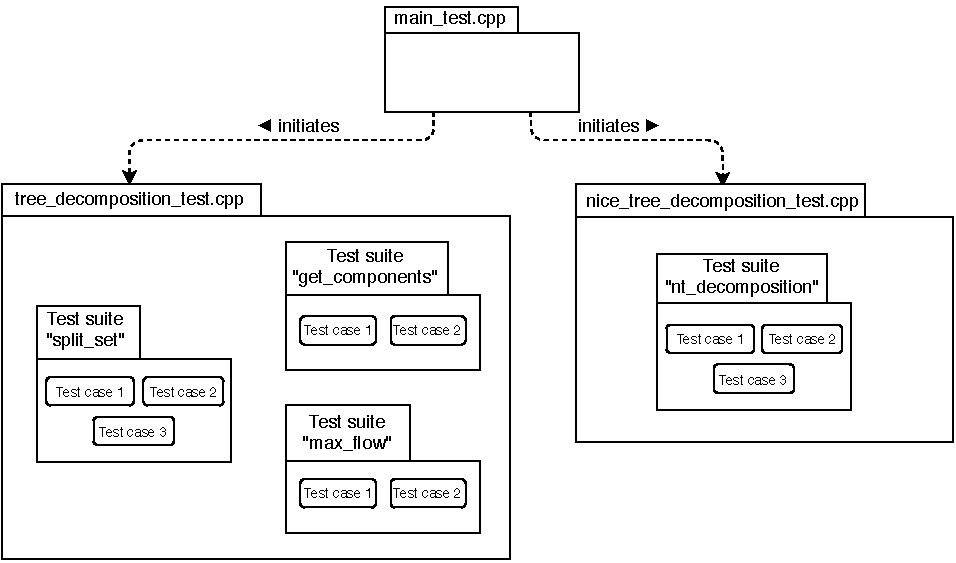
\includegraphics[width=12cm]{img/test-structure.pdf}
 	\caption[Structure of tests used in our library extension]{Structure of tests used in our library extension.}
 	\label{fig:test_structure}
\end{figure}

\subsection{Fixtures}\label{ssec:fixtures}
In general terms a test fixture or test context is the collection of one or more of the following items, required to perform the test~\cite{boost_test_fixtures}:

\begin{itemize}
	\item Preconditions.
	\item Particular states of tested units.
	\item Necessary clean-up procedures.
\end{itemize}

The main advantage of fixtures is in their re-usability---say, we want to test several different functions on the same graph. Instead of re-declaring the graph in each function (which is against DRY\footnote{DRY (Don't repeat yourself) principle is a principle that focuses on reducing the repetition of information of all kind (e.g., code duplication).} principle), we will define the graph only once in the fixture and then pass the fixture inside a \emph{Test suite}, where it can be used in multiple test cases.

In BTL, a fixture is represented by a \texttt{struct}. Fixture data are stored in~\texttt{struct} as \emph{members}. Each time a fixture is required by a \emph{Test suite}, procedure \texttt{setup} is initiated (in case of BTL, the constructor of \texttt{struct}). After finishing all test cases in a \emph{Test suite}, procedure \texttt{teardown} is initiated (destructor of \texttt{struct}).

In our case, fixtures are mostly used to define multiple graphs or decompositions and their bags, that will be used in a \emph{Test suite}. Example of a such a fixture is shown in \autoref{lst:fixtures}.

\begin{listing}[H]
	\inputminted[tabsize=2,breaklines,bgcolor=codebg]{c++}{snippets/fixtures.m}
	\caption[Example of a \emph{fixture} that is \uv{injected} into a \emph{Test suite}]{Example of a \emph{fixture} that is \uv{injected} into a \emph{Test suite}.}
	\label{lst:fixtures}
\end{listing}

\subsection{Testing of the functions}
In each test case we are testing the result of a single call of a function that is being tested. Take a testing of helper function \texttt{max\_flow\_sep} (described in \autoref{ssec:retrieving_separation}) as an example---inside the test case we are asserting that the retrieved separation has a correct size and contains expected vertices (see \autoref{lst:sep_test}).

\begin{listing}[H]
	\inputminted[tabsize=2,breaklines,bgcolor=codebg]{c++}{snippets/sep_test.m}
	\caption[Testing of the function \texttt{max\_flow\_sep}]{Testing of the function \texttt{max\_flow\_sep}.}
	\label{lst:sep_test}
\end{listing}

Some of the functions are a bit too complex to test them in such a simple manner---one of those functions is \texttt{tree\_decomposition}. As we learnt in \autoref{sec:td_implementation}, its purpose is to find the decomposition of a given graph. However decompositions are not generally unique, there can be many different decompositions of the graph (e.g., trivial decomposition contains all vertices in a single root node). That is why instead of comparing retrieved decomposition with a reference decomposition, we will test, if it meets following conditions that basically define tree decompositions:

\begin{enumerate}
	\item Width of the decomposition is at most $3k+4$.
	\item Every vertex is in at least one bag.
	\item Every edge is in at least one bag.
	\item Set of nodes containing any vertex $v$ induces a connected component.
	\item Decomposition is a tree.
\end{enumerate}

If all of the listed conditions are met, the decomposition is valid. The same approach is used when testing the function \texttt{nice\_tree\_decomposition} (more conditions are added since a nice tree decomposition is more strict than general decomposition).

\subsection{Continuous integration}\label{ssec:ci}
Since our library extension is hosted on GitLab, managing continuous integration is relatively easy. With each push or merge request GitLab runs a pipeline of scripts to build and test our library extension. The pipeline and its content is defined in file \texttt{.gitlab-ci.yml} located in the root of the project.
\newpage
\noindent Our pipeline is divided into two stages:
\begin{enumerate}
	\item \textbf{Build}. In this phase all of the source files are compiled using the \texttt{make compile} command.
	\item \textbf{Test}. In this phase the tests are run using the \texttt{make test} command.
\end{enumerate}
If any of these two stages fails, GitLab prevents merging into \emph{master} branch until the errors are fixed and both of the stages pass (this is a default behaviour for protected branches~\cite{gitlab_ci}). This prevents from pushing faulty code into the \emph{master} branch. The status of the pipeline can be viewed on GitLab website (see \autoref{fig:pipeline}).

\begin{figure}[H]
	\centering
 	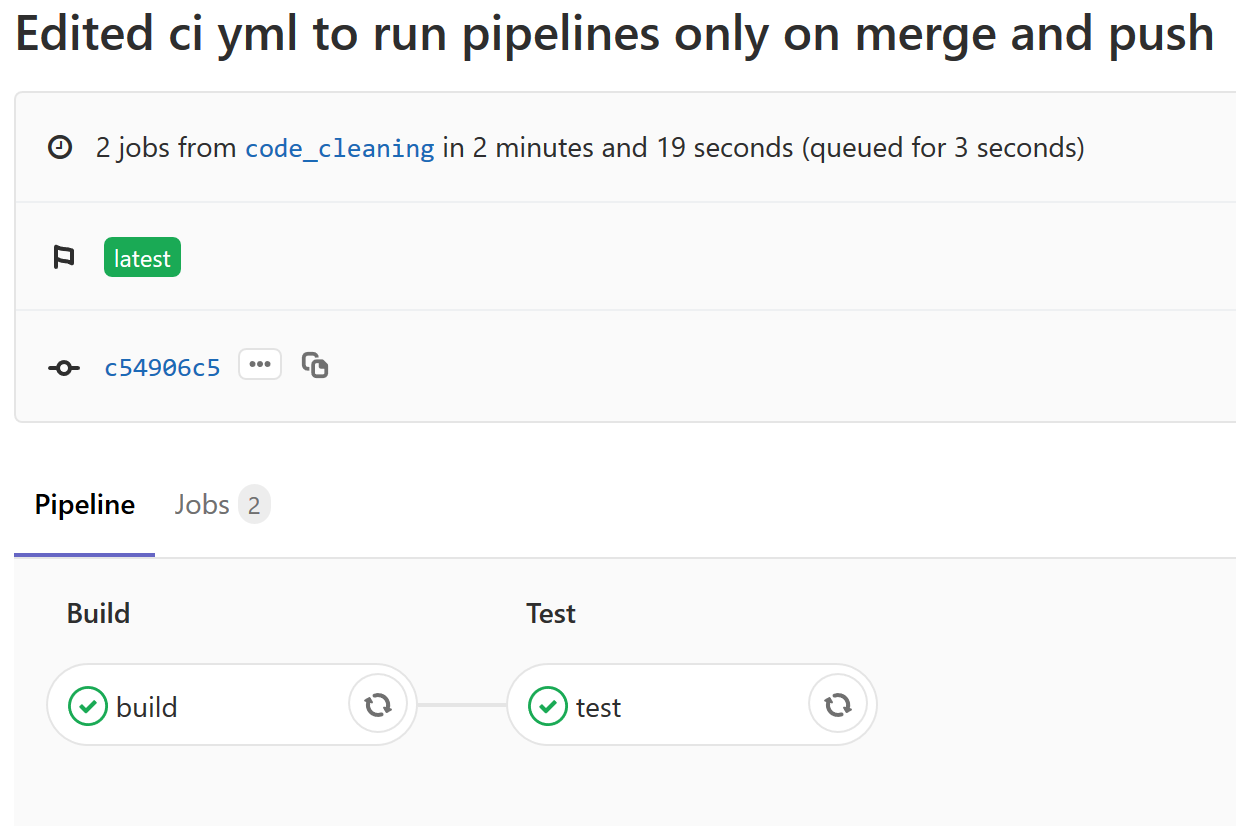
\includegraphics[width=1\textwidth]{img/pipeline}
 	\caption[Status of the pipeline and its stages]{Status of the pipeline and its stages.}
 	\label{fig:pipeline}
\end{figure}

\subsection{Fulfilling of the requirements}\label{ssec:fulfilling_requirments}
In this subsection we will review the fulfilment of the functional and non-functional requirements that we have defined in \autoref{sec:requirment_specification}. Each requirement will be discussed in a separate paragraph:\bigskip

\noindent\textbf{Requirement F1}. Algorithm for obtaining a tree decomposition was successfully implemented in a file \texttt{src/tree\_decomposition.hpp}. Its implementation is discussed in \autoref{sec:td_implementation}.\newpage

\noindent\textbf{Requirement F2}. Algorithm for obtaining a nice tree decomposition from general tree decomposition was successfully implemented. General decomposition is supplied to the function as an input (see \autoref{sec:ntd_implementation}). File \texttt{nice\_src/\-tree\_decomposition.hpp} contains implementation of the algorithm.\bigskip

\noindent\textbf{Requirement F3}. Algorithm for solving the maximum weighted independent set was chosen as a demonstration of usage of dynamic programming over a tree decomposition. The implementation of the algorithm is located in \texttt{src/max\_weighted\_independent\_set.hpp}. For more details see \autoref{sec:mwis}.\bigskip

\noindent\textbf{Requirement F4}. Every function defined in our library extension uses template parameters, so that user is not bound to certain type of graph. This also applies to other data structures, e.g., \emph{Property Map} representing bags of the decomposition.\bigskip

\noindent\textbf{Requirement F5}. Exceptions are thrown only if the user provides an input, that would cause an infinite loop---e.g., a decomposition that is not a tree in the function \texttt{src/max\_weighted\_independent\_set.hpp}. Incorrect template arguments cause a compilation error thanks to usage of concept checks.\bigskip

\noindent\textbf{Requirement F6}. Algorithm \texttt{nice\_tree\_decomposition} is not bound to any algorithm for obtaining a tree decomposition. Instead, tree decomposition is supplied as an input (therefore avoiding the decision to use specific decomposition algorithm) as opposed to retrieving the decomposition as a part of the~algorithm.\bigskip

\noindent\textbf{Requirement N1}. Our library extension follows most of the conventions used by BGL, e.g., code structure, naming conventions (words separated by \uv{\_} instead of using camel-case) or indentation. As it is customary for BGL, each of the algorithms is implemented and defined in a header-file.\bigskip

\noindent\textbf{Requirement N2}. Each of the algorithms used in our library extension uses only C++ Standard Library or Boost libraries---no other third-party libraries were used.\bigskip

\noindent\textbf{Requirement N3}. Documentation of the interface is provided in form of HTML pages generated by Doxygen (see \autoref{sec:documentation}).\bigskip

\noindent\textbf{Requirement N4}. Algorithms and helper-functions used in those algorithms are tested by BTL (note that not every helper-function is tested, because they are either a wrapper or they cannot be tested). Tests are located in directory \texttt{test/} and they are initiated by \texttt{test/main\_test.cpp}. These tests are also a part of continuous integration (see \autoref{ssec:ci}).
\section{Documentation}\label{sec:documentation}
Documentation of this library is supposed to serve as a reference guide for users, that will be using the functions provided by our extension. This is the~main reason why only the interfaces of those functions are described and not the helper-functions, since they are irrelevant to the user. Documentation is generated by Doxygen---a tool frequently used for documentation of C++ source codes.

It can generate an on-line documentation browser (in HTML) and/or an off-line reference manual from a set of documented source files. The documentation is extracted directly from the sources, which makes it much easier to keep the documentation consistent with the source code~\cite{doxygen}.

Source files have to be described with specific annotations\footnote{Annotation is a special type of comment block that contains additional or meta-information in the source code.} in order to be documented (see \autoref{lst:annotation} for an example).

\begin{listing}[H]
	\inputminted[tabsize=2,breaklines,bgcolor=codebg]{c++}{snippets/annotation.m}
	\caption[Annotation of the function \texttt{tree\_decomposition}]{Annotation of the function \texttt{tree\_decomposition}.}
	\label{lst:annotation}
\end{listing}

Generated documentation is located in a directory \texttt{doc/html/} and available from \texttt{doc/index.html}, which redirects to a list of functions provided by our library extension. For each function there is a description of its purpose, used libraries, (template) parameters, and the return value. Segment of documented function \texttt{tree\_decomposition} is shown in \autoref{fig:documentation}.

\begin{figure}[H]
	\centering
 	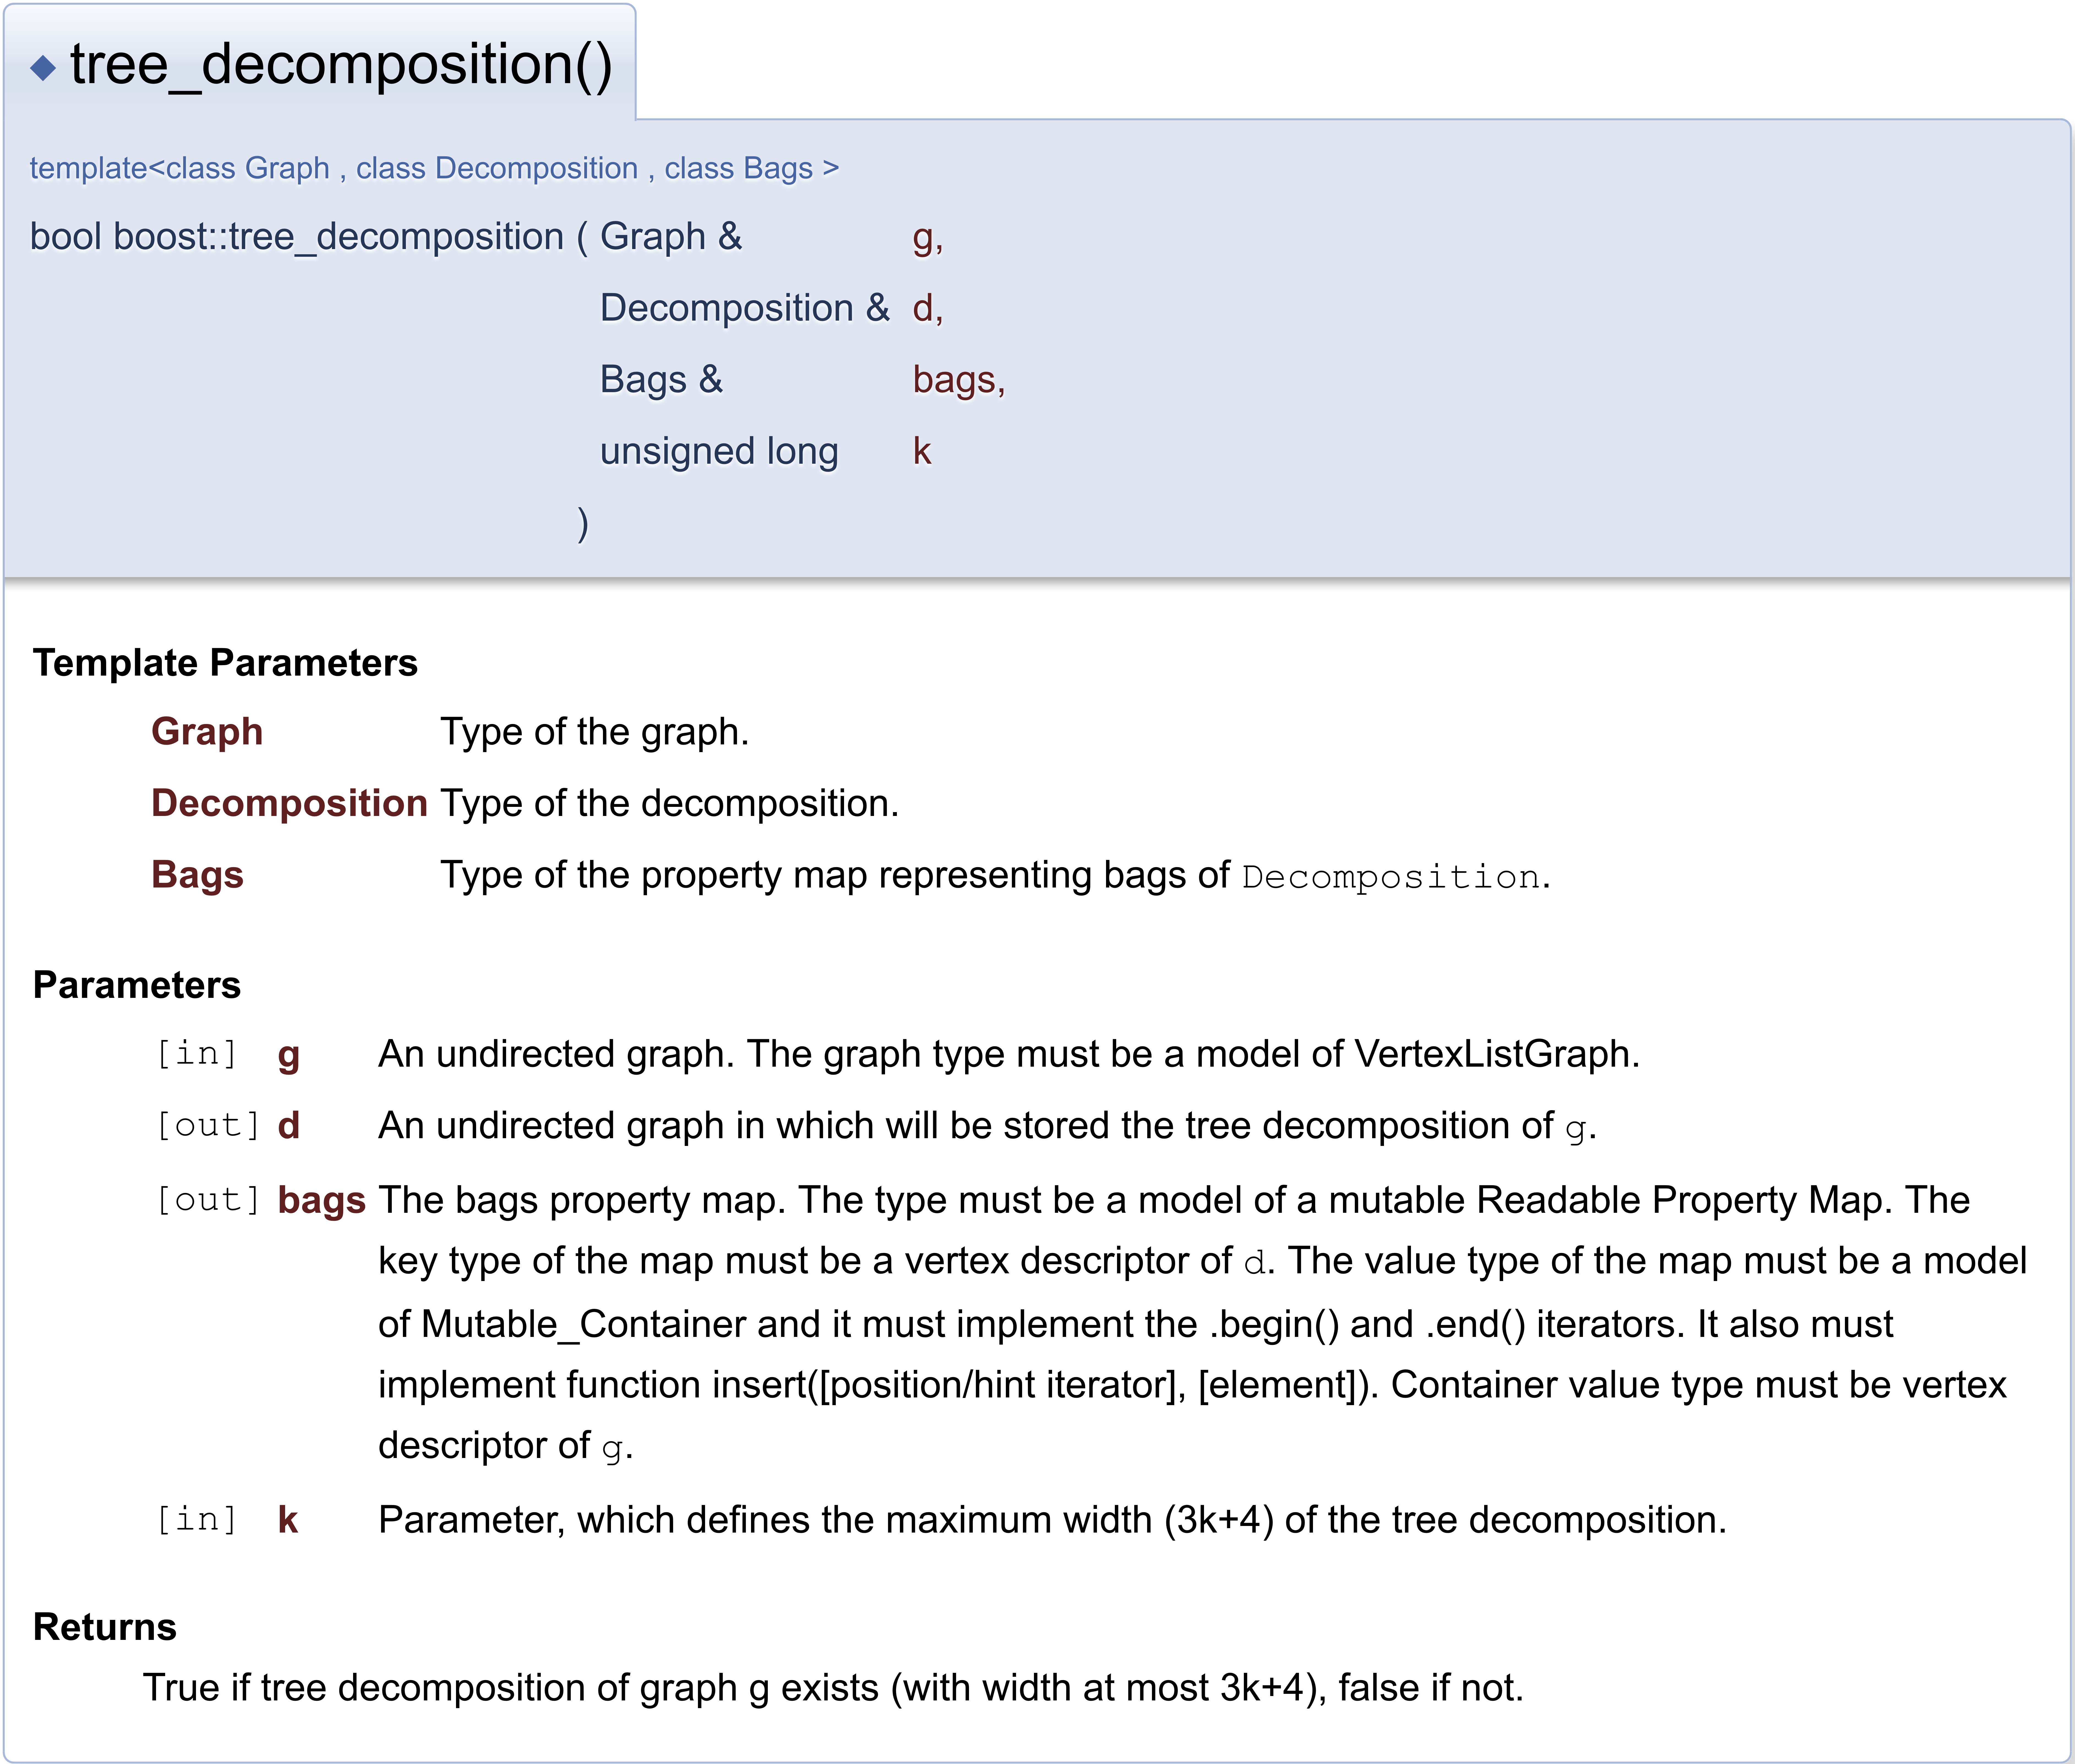
\includegraphics[width=1\textwidth]{img/documentation}
 	\caption[Example of the documentation generated from annotation presented in \autoref{lst:annotation}]{Example of the documentation generated from annotation presented in \autoref{lst:annotation}.}
 	\label{fig:documentation}
\end{figure}

\setsecnumdepth{part}
\chapter{Conclusion}
The goal of this thesis was to extend the C++ Boost Graph Library with algorithms for obtaining a general/nice tree decomposition along with algorithm, that demonstrates the usage of dynamic programming over a tree decomposition, which was successfully fulfilled along with all of~the~functional and non-functional requirements (as we discussed in \autoref{ssec:fulfilling_requirments}).

Heavy emphasis was put on genericity of the functions provided by our library extension, which was achieved using the C++ templates and concepts defined by BGL---functions can be used with various types of graphs and data~structures.

There is lot of space for further improvement of our library extension:

\begin{itemize}
	\item Optimization of used algorithms.
	\item Provide more algorithms that use a tree decomposition to improve their performance.
	\item Make the parameter $k$ of the function \texttt{tree\_decomposition} optional.
	\item Implement exact FPT algorithm for obtaining a tree decomposition, allowing the user to choose, whether exact or approximate FPT algorithm should be applied. 
\end{itemize}

This work, including the thesis, source-codes, and documentation is uploaded on the attached SD card. The work is also available from faculty GitLab in repository:\\ \url{https://gitlab.fit.cvut.cz/kralva10/treewidth-support-for-bgl}

%\bibliographystyle{iso690}
%\bibliography{bibliographyfile}
\printbibliography

\setsecnumdepth{all}
\appendix

\chapter{Acronyms}
% \printglossaries
\begin{description}
	\item[2D] Two-Dimensional
	\item[BCCL] Boost Concept Check Library
	\item[BGL] Boost Graph Library
	\item[BTL] Boost Test Library
	\item[DRY] Don't Repeat Yourself
	\item[FPT] Fixed-Parameter Tractable
	\item[GCC] GNU Compiler Collection
	\item[GNU] GNU's Not Unix
	\item[HTML] HyperText Markup Language
	\item[OS] Operating System
	\item[PNG] Portable Network Graphics
	\item[PRNG] Pseudo-Random Number Generator
	\item[SD] Secure Digital
	\item[SDLC] Software Development Life Cycle
	\item[STL] Standard Template Library
	\item[TV] Television
	\item[UML] Unified Modelling Language
\end{description}

\chapter{Installation instructions}
In this appendix we will describe contents, requirements, and usage of our library extension.

\section{Contents}
Our library extension consists of three header files located in directory \texttt{src/}:
\begin{itemize}
	\item \texttt{tree\_decomposition.hpp} containing a function for retrieving a tree decomposition.
	\item \texttt{nice\_tree\_decomposition.hpp} containing a function for retrieving a nice tree decomposition.
	\item \texttt{max\_weighted\_\-independent\_set.hpp} containing a function that computes a maximum weighted independent set.
\end{itemize}

Documentation of those three header files is located in \texttt{doc/index.html}. Examples can be found in directory \texttt{example/}. Lastly, \texttt{Makefile} which is used to build example and tests is in the root of the project.


\section{Requirements}
Our library extension was developed on Linux OS using the GCC compiler (version C++14) and GNU Make. Successful compilation with older versions of GCC or different OS is not guaranteed.

Provided header files require \emph{Boost 1.72.0}\footnote{\url{https://www.boost.org/users/history/version_1_72_0.html}} library (older versions might not be compatible). Library can be installed using the command:

\mint{bash}|sudo apt-get install libboost-dev|

\section{Usage example}
In order to help the users to get more familiar with our library extension we also provide examples of usage. The file with the examples is located in \texttt{example/example.cpp} and contains a sample graph on which are applied functions that we presented earlier in this chapter.

The form of the output of the example depends on the boolean variable \texttt{SAVE\_GRAPHS}. If it is set to \emph{false}, the graphs (e.g., constructed tree decompositions) will be printed in text form into \texttt{stdout}. Otherwise, the graphs will be saved into \emph{.dot}\footnote{DOT is a graph description language used to represent graphs in a simple text form.} files in the \texttt{example/} directory. In addition, if the user has installed the \emph{Graphviz} library\footnote{Available from \url{https://www.graphviz.org/download/}}, PNG files will be created from \emph{.dot} files using the \texttt{dot} command. \emph{Graphviz} library can be installed using the command:

\mint{bash}|sudo apt-get install graphviz|

\section{Make commands}
As we mentioned, to compile and run our library extension together with example or tests we are using GNU Make. See \autoref{tab:make_commands} for available \texttt{make} commands that can be run from the root of the project.

\begin{table}[h]
\centering
\begin{tabular}{|l|l|}
\hline
\textbf{Command} & \textbf{Usage} \\ \hline
\texttt{make all} & Compile both example and tests. \\
\texttt{make compile} & Same as \texttt{make all} \\
\texttt{make doc} & Generate documentation \tablefootnote{Doxygen version 1.8.17 or newer required.} \\
\texttt{make run} & Compile and run example. \\
\texttt{make test} & Compile and run tests. \\
\texttt{make help} & Show help. \\
\texttt{make run} & Clean binaries and \texttt{obj/} directory. \\ \hline
\end{tabular}
\caption[Available \texttt{make} commands used to build example and tests]{Available \texttt{make} commands used to build example and tests.}
\label{tab:make_commands}
\end{table}

\chapter{Contents of enclosed SD card}

%change appropriately

\begin{figure}
	\dirtree{%
		.1 README.md\DTcomment{the file with SD card content description}.
		.1 project\DTcomment{the directory with the source files}.
		.2 doc\DTcomment{the directory with documentation}.
		.2 example\DTcomment{the directory with examples of usage}.
		.2 src\DTcomment{the directory of source codes}.
		.2 test\DTcomment{the directory with tests}.
		.2 thesis\DTcomment{the directory of \LaTeX{} source codes of the thesis}.
		.1 text\DTcomment{the thesis text directory}.
		.2 thesis.pdf\DTcomment{the thesis text in PDF format}.
	}
\end{figure}

\end{document}
